
% !TEX root = DesignDocument.tex

\chapter{Design  and Implementation}

\section{Systems Goals}
\begin{itemize}
	\item Provide an easy-to-use 2D simulation environment
	\item Simulate realistic physics as best as possible
	\item Support easy modification and extension of the simulation
	\item Allow saving and loading entire simulation state
	\item Allow for design of custom robots to use in the simulation
\end{itemize}

\section{System Overview and Description}
There are six major components in this system
\begin{itemize}
	\item Application core
	\item General User Interface
	\item World Visualization
	\item Physics Engine
	\item File Read/Write
	\item Plugin System
\end{itemize}
See figure \ref{fig:systemdiagram} for an overview representation of where the components reside in the application and what other components they connect to.

\begin{figure}[tbh]
\begin{center}
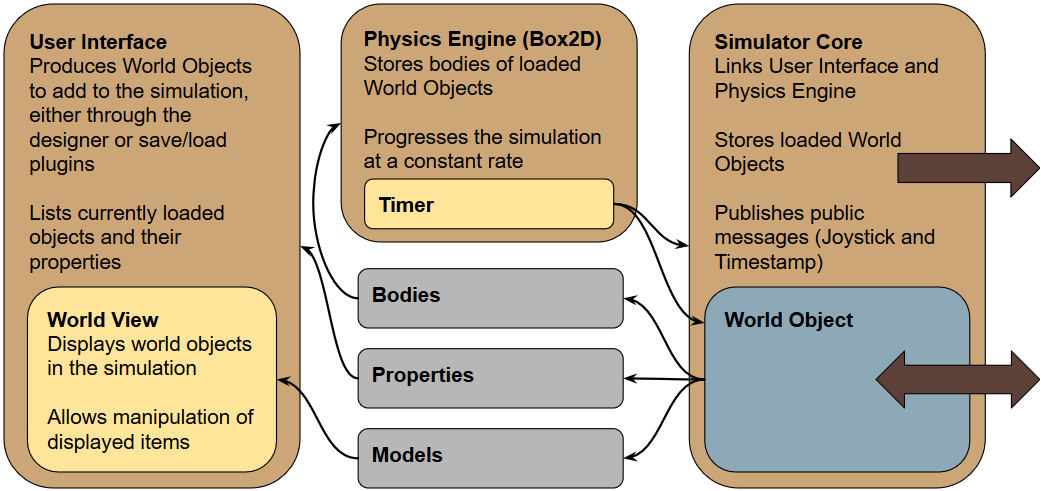
\includegraphics[width=0.9\textwidth]{./images_design/sysarch2_flow}
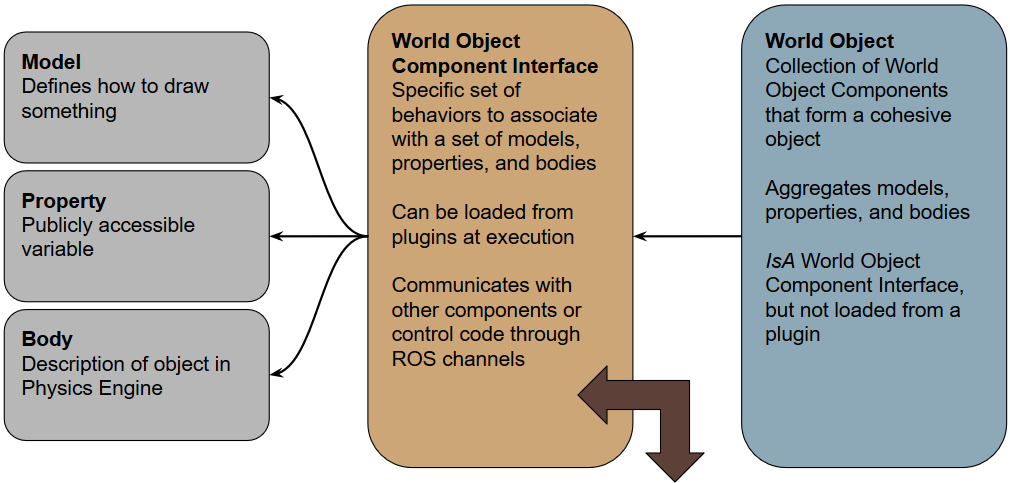
\includegraphics[width=0.9\textwidth]{./images_design/sysarch2_datatypes}
\end{center}
\caption{A visual representation of the system architecture; both the basic data types and data flow\label{fig:systemdiagram}}
\end{figure}

\subsection{Application Core}
The Application Core has the job of organizing the rest of the system. It connects all of the events generated by the other components and keeps track of all simulated objects. It is also responsible for adding and removing simulated objects when commanded to.

Explained in more detail below, anything simulated in the application can be represented in the World Object class. The World Object exposes functions to
\begin{itemize}
	\item Add/Remove itself from the physics engine
	\item Obtain its Models for drawing on screen
	\item Obtain its list of Properties
\end{itemize}

Models and Properties are fully defined below as well.

\subsection{Physics Engine}
The Physics Engine is the backbone of the simulation. The main purposes of the Physics Engine are
	\begin{itemize}
		\item Track what objects are part of the simulated world
		\item Step the simulated world at a regular rate
		\item Notify simulated objects when the world updates
	\end{itemize}
Forces can be applied to the simulated objects at any point in time, by any part of the application. The Physics Engine does not concern itself with where the forces originate, just the effects of them.
 
\subsection{User Interface}
The User Interface consists of all portions of the UI which are not the visualization of what is actually being simulated. The UI is responsible for things like providing the user with ways to load and save files, start and stop the simulation, and edit the properties of the simulated objects.

While the visualization of the simulated activity is, technically speaking, part of the UI, it is connected to the rest of the UI through a single interface. This allows it to be developed independently and means the rest of the UI should be agnostic to the details of how it looks and behaves. We will reference the visualization in this document with terms such as "World Visual", or "Visualization Widget".

\subsection{World Visualization}
The World Visualization is a widget in the UI which is responsible for portraying the simulated activity. Its communication is strictly with the general UI, as it is a child object of it. The UI is expected to tell this visual when objects are added and removed, as well as what models belong with those objects.

\subsection{File Read/Write}
The File Read/Write component is utilized by the general UI. When the user selects a file, the Read/Write component loads or saves a world object or collection of world objects in that file. If the file is malformed, it returns an error that the UI can display. File handlers are loaded from plugins on startup; the base project includes a save/load handler which utilizes JSON format, and a loader which can convert images to sets of World Objects.

\subsection{Plugin System}
The Plugin System keeps the core application logic separate from the specific capabilities of the simulated objects. Plugins provide the components which make up the objects simulated. Using this design allows users to write their own components for the simulation if some desired feature is missing.

\section{Technologies Overview}
\subsection{C++}
	The entire application is written using the C++ programming language. Reference material for the syntax and libraries provided as part of the language can be found at \url{http://en.cppreference.com/w/}. The most recent standard used by this project is C++11.
	
\subsection{Qt}
	Qt is a cross-platform development framework and library. It is utilized in this project for a couple of specific features it provides
	\begin{itemize}
		\item Event Loop
		\item QObjects
		\item Signals and Slots
		\item Plugins
		\item Widgets Library
		\item Graphics Framework
	\end{itemize}
	Information about the project can be found at \url{http://doc.qt.io/}. Some of the core concepts of these features are described in the following sections.
	
	An example containing QObjects and Signals and Slots can be seen in listing \ref{lst:qobjexample} below.
	
\subsubsection*{Event Loop}
	The central part of Qt is the Event Loop. When a Qt application is started, it generally enters an event loop which spins during idle time. When an event happens, it is queued until the start of the next iteration of the event loop. During each iteration of the event loop, all pending events are delivered to their receivers to be handled.
	
	\begin{lstlisting}[caption={Pseudocode for the Qt Event Loop}]
while(application_running)
{
	for(event in event_queue)
		handleEvent(event)
	Remove handled events
}
	\end{lstlisting}
	
	Many events are user-generated by actions such as clicking buttons, typing text, and resizing windows. Other events may take the form of cross-thread communication through Signals and Slots.
	
\subsubsection*{QObject}
	QObjects are the base type of anything residing in the Qt event framework. Similarly to how all Java types inherit Object, all Qt objects inherit QObject. There are two parts to QObject inheritance.
	\begin{enumerate}
		\item Inheriting QObject will add a number of common functions, signals, and slots to a type. When QObjects are instantiated, they can be given a parent QObject. When a parent QObject is destroyed, it will automatically destroy all of its children.
		\item The Q\_OBJECT macro must be placed in the \lstinline|private| portion of the class definition. At compile time, the Qt Meta Object Compiler (or MOC) is run before the standard C++ compiler. The MOC finds this macro and other Qt-specific keywords and generates standard C++ files which a normal compiler, such as g++, can use.
	\end{enumerate}
	
	Limitations on inheritance of QObject
\begin{enumerate}
	\item QObject cannot be inherited in a templated class
	\item If multiple types are inherited, QObject (or a type that isa QObject) must be the last type inherited
	\item QObject cannot be virtually inherited, so the diamond inheritance problem cannot be resolved if all types are QObjects
\end{enumerate}
	
\subsubsection*{Signals and Slots}
Signals and Slots allow programmers to define custom events and event handlers in their objects. 

A Signal is a public method of a QObject which has no definition. (The definition is added by the MOC). Instantiated QObjects can emit signals at any point in time. Signals may have parameters, and when the object emits a signal with parameters, it will fill them with data.

A Slot is a public, protected, or private method of a QObject. It must have a full definition just like any other method. (In many cases, it can be treated exactly as if it were a regular method.)

There are two main limitations on Signals and Slots
\begin{enumerate}
	\item All parameters MUST be pass-by-value. This allows all data to be copied, preventing race conditions when signals trigger slots in other threads.
	\item Custom types passed as parameters in signals and slots must be known to the Qt Meta-Object System. See documentation on the qRegisterMetaType() function for more information on how this works.
\end{enumerate}

At runtime, applications can connect the signals of instantiated QObjects to the slots of any other instantiated QObjects. When a QObject emits a signal, any slots that it is connected to will be called.


\begin{lstlisting}[language=C++, caption={Example of QObjects with parenting, Signals and Slots, and connections.\label{lst:qobjexample}}]
class foo : public QObject
{
	Q_OBJECT
public:
	//Construct with optional parent QObject
	foo(QObject* parent=nullptr) : QObject(parent){}

//Keyword known to MOC
//All signals are public methods
signals:
	void somethingHappened();
	void otherThingHappened(int);

//Another MOC keyword. Slots can be public, private, or protected
public slots:
	void reactToAnotherThing(int x)
	{
		cout << "Another thing: " << x << endl;
	}
};

class bar : public QObject
{
	Q_OBJECT
public:
	//Construct with optional parent QObject
	bar(foo* parent) : QObject(parent)
	{
		//Connect events between objects
		//Note that events and handlers have the same function signature	
		
		//When somethingHappened() is emitted by 'parent'
		//Do reactToSomething() in 'this'
		connect(parent, &foo::somethingHappened,
		        this, &bar::reactToSomething);
		
		//When otherThingHappened() is emitted by 'parent'
		//Do reactToOtherThing() in 'this'
		connect(parent, &foo::otherThingHappened,
		        this, &bar::reactToOtherThing);
		
		//When anotherThingHappened() is emitted by 'this'
		//Do reactToAnotherThing() in 'parent'
		connect(this, &bar::anotherThingHappened,
                parent, &foo::reactToAnotherThing);
	}

//Keyword known to MOC
//All signals are public methods
signals:
	void anotherThingHappened(int);	

//Another MOC keyword. Slots can be public, private, or protected
private slots:
	void reactToSomething()
	{
		cout << "Something happened!" << endl;
	}
	
	void reactToOtherThing(int x)
	{
		cout << "Reacting to other thing: " << x << endl;
		
		//Send a signal back to 'parent' object
		emit anotherThingHappened(x+1);
	}
};

int main()
{
	//Put a 'bar' on the
	foo* f = new foo();
	bar* b = new bar(f);
	
	//This will delete b as well because 
	//b is a child of f
	delete f;
}
\end{lstlisting}

\subsection{Box2D Physics}
The Box2D library is used as the basis of the Physics Engine for this simulation. It is a C++ library which can be used for realistic physics simulation and collision detection. The Box2D project is hosted on github at this location \url{https://github.com/erincatto/Box2D}.

When working with a Box2D simulation, there are a number of types that are used.
\begin{itemize}
	\item b2World: Container for everything being simulated and all extra simulation information. Bodies and Joints are added directly to the World to be simulated.
	\item b2Body: Container for physics information for one specific element of the simulation. Bodies are made up of any number of Fixtures, which are held relative to each other as the body moves. Bodies contain information such as mass, inertia, velocity, etc. Bodies can also be acted upon by forces or impulses.
	\item b2Fixture: Fixtures are used to attach shapes to a Body. Each fixture is used to attach a single shape.
	\item b2Shape: Abstract base type of any shape. Various shapes are supported by Box2D, but this project utilizes mainly b2PolygonShape and b2CircleShape.
	\item b2Joint: Joints are used to constrain how bodies move relative to each other. Many types of joints exist in Box2D, some examples are rigid, revolute, prismatic, and motor.
\end{itemize}

\subsection{ROS}
As mentioned a number of times previously, this simulation supports communication with external applications through ROS, the Robotics Operating System. Information on ROS can be found at \url{http://www.ros.org/}. The version of ROS targeted for this project is ROS 2 Ardent Apalone.

The core application itself has minimum communication through ROS, it mainly starts a ROS listener thread so that messages can be received. The bulk of the message sending and receiving is done by the plugin components which make up the objects being simulated. There are two messages sent from the core application -- A timestamp message to indicate the time passed in the simulation and joystick control messages from the virtual joystick.

\newpage
 \section{Architecture and System Design} 	
 \subsection{Design Decisions}
  	The simulation underwent a number of design changes during its development. This section will discuss what drove the major design decisions associated with this project.
 \subsubsection*{User Experience}
	Because this application is mainly for students just being introduced to robotics and will be a tool for education, we wanted to make the simulator as user friendly as possible. We decided to try for a video game-like feel, as most individuals are familiar with video games which would make it easy to learn. 
	
	The biggest design decision we had to make for the user experience aspect of the project was whether we wanted to use a single window for everything (simulation, robot builder and map builder) or if we wanted to have multiple windows. We began with a few concepts and wire frames. 

\begin{figure}
\begin{subfigure}{0.5\textwidth}
	\begin{center}
	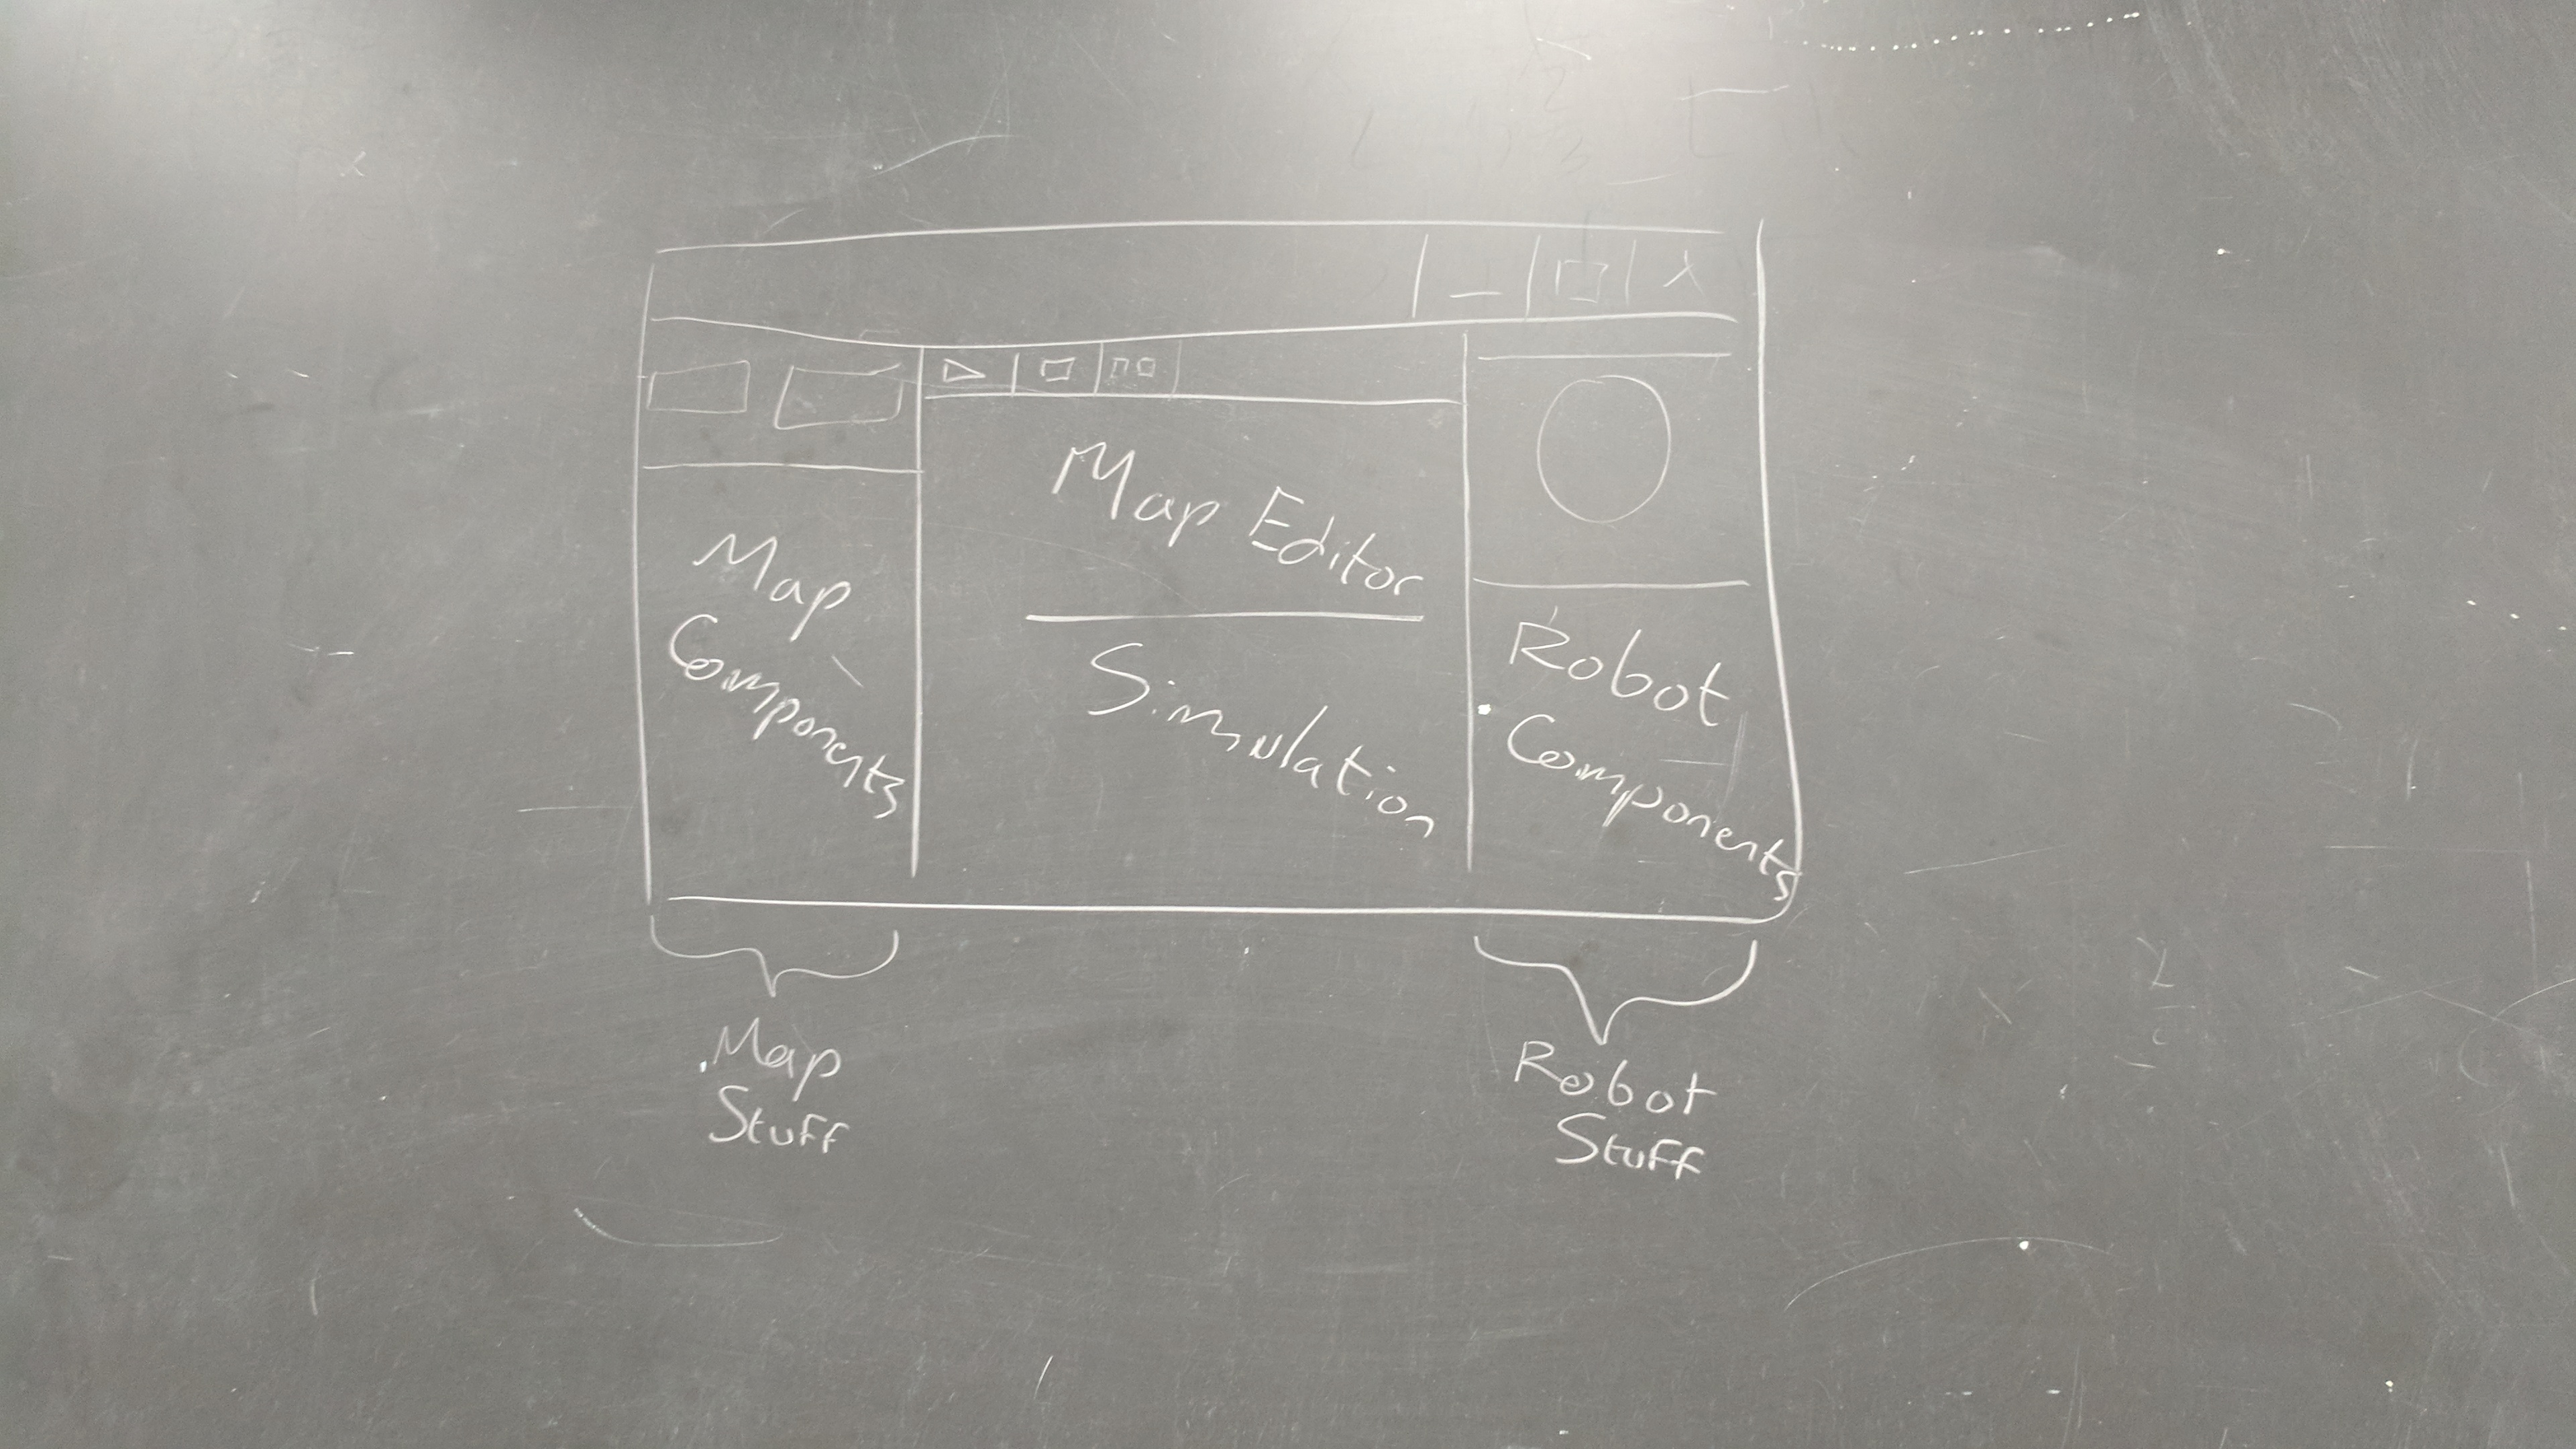
\includegraphics[width=0.9\textwidth]{./images_design/Sams.jpg}
	\caption{Single Window Concept}
	\label{fig:singlewindowconcept}
	\end{center}
\end{subfigure}
\begin{subfigure}{0.5\textwidth}
	\begin{center}
	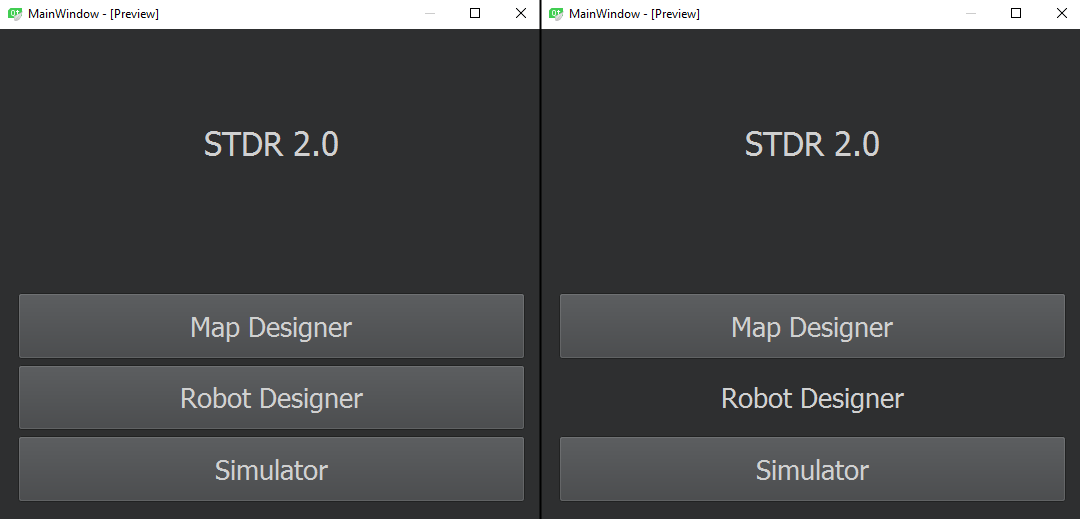
\includegraphics[width=0.9\textwidth]{./images_design/MainScreen.png}
	\caption{Multi-Window Start Window}
	\label{fig:mwindowStart}
	\end{center}
\end{subfigure}

\begin{subfigure}{0.5\textwidth}
	\begin{center}
	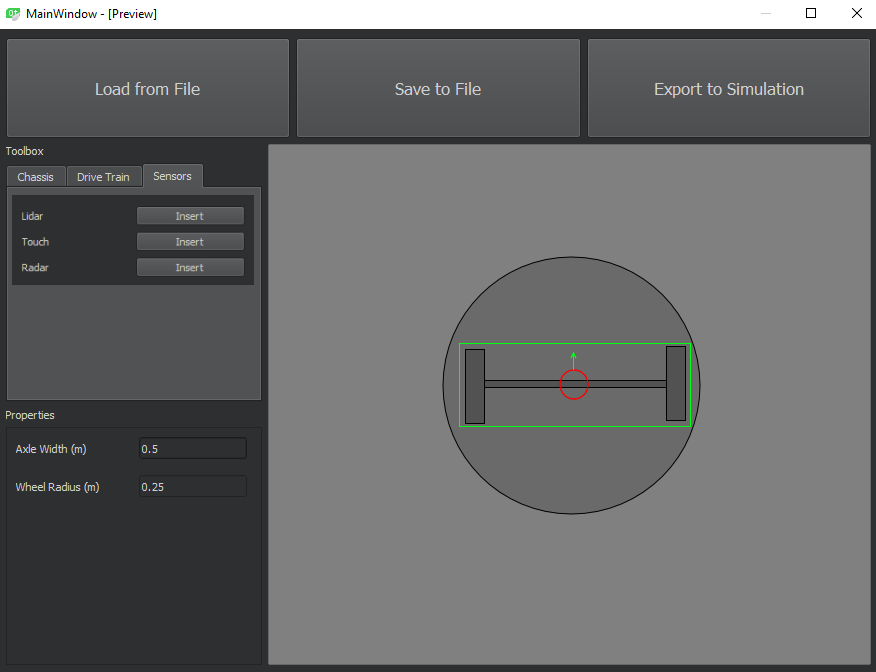
\includegraphics[width=0.9\textwidth]{./images_design/RobotDesign.png}
	\caption{Multi-Window Robot Designer}
	\label{fig:mwindowRobot}
	\end{center}
\end{subfigure}
\begin{subfigure}{0.5\textwidth}
	\begin{center}
	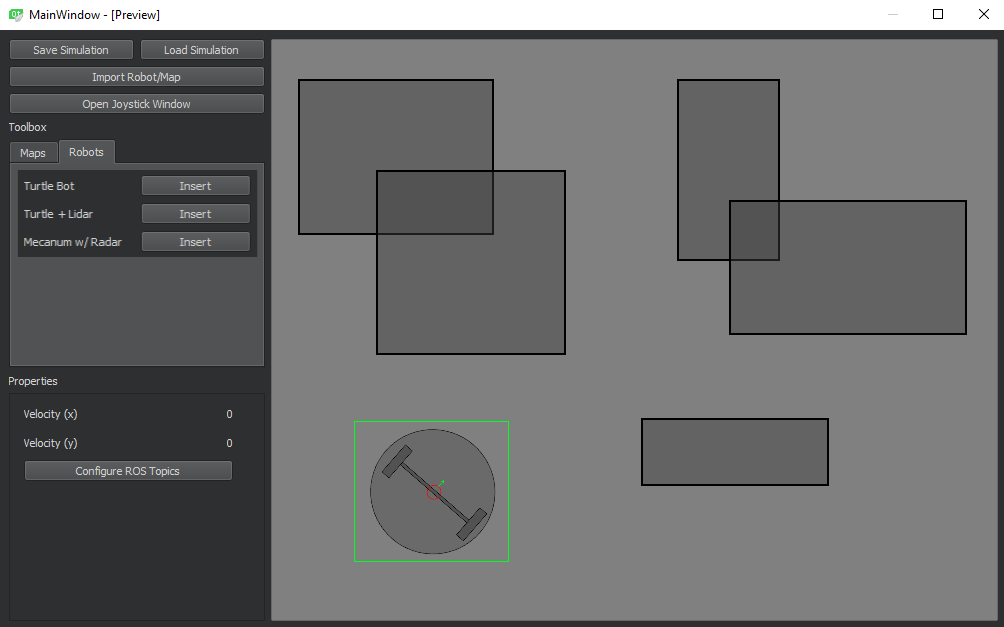
\includegraphics[width=0.9\textwidth]{./images_design/Simulation.png}
	\caption{Multi-Window Simulation}
	\label{fig:mwindowSimulation}
	\end{center}
\end{subfigure}
\caption{Example UIs presented to the Client}
\end{figure}
	
	The chalkboard drawing \ref{fig:singlewindowconcept} shows an early concept for a single window interface, while the wireframes \ref{fig:mwindowStart}, \ref{fig:mwindowRobot}, and \ref{fig:mwindowSimulation} show an idea for a multiple window interface. 

We chose to go with the single-window application both because it looks 'cleaner' and because there would be little advantage to building our application with multiple windows. It is anticipated that the user would not need to use the designer during a simulation, or the simulation during the design process; so it makes little sense to make them accessible simultaneously.  
 
 
 \subsubsection*{User Interface}
 	When building a cross-platform user interface in C++, there are only a few options available. When discussing this, the following ideas were brought up: Pure OpenGL, Qt QML, and Qt Widgets. The final decision was Qt Widgets, which will be discussed below.
 	
 	A pure OpenGL solution was not selected due mainly to the difficulty of implementation and the amount of work that would have to go into a UI of that nature. If using Qt were not an option, pure OpenGL may have been selected; however, having the Qt library available makes it hard to justify the amount of extra development that a pure OpenGL solution would add.
 	
 	When writing a UI in Qt, there are two main options for the core library: Widgets and QML. Qt Widgets has been around longer and is generally used to produce applications that look and feel 'like a desktop program'. The Widgets library contains many commonly used pieces which can be organized into a UI, similarly to how C\# Forms or Java Swing works. Qt QML is a newer library which is being actively developed with Qt. QML separates the UI entirely from the business logic by running the UI in a custom javascript interpreter. The main advantages to QML are that it's very easy to develop QML UIs without any business logic and it's currently receiving the bulk of support in new versions of Qt. QML would have been the first choice for the project UI, but it is difficult to use on a freshly installed system. Widgets projects require just a set of shared objects to run, but QML projects require a number of shared objects as well as some basic QML code files which are parsed at runtime. These additional files are not usually present in the base library installation of Qt, so using QML would have meant that the end user would need to resolve extra dependencies to run the application.
 	
 	\subsubsection*{World Visualization}
 	Within the Qt Widgets library, there are a number of different ways build a widget with a drawing canvas that shapes can be shown on. The most primitive method is to create an OpenGL drawing window which is contained in the widget. The other main option is to use the Qt Graphics Framework, which is an abstraction layer for drawing 2D objects on a background with OpenGL.
 	
 	Again, it was decided that the pure OpenGL solution would add unnecessary development time, and an alternative should be used. Not only does the graphics framework provide easy methods for drawing primitive shapes on a canvas, but it also allows for parent-child relationships between the models, which in turn allows shapes to be defined with relative transforms to each other instead of everything needing to be in world coordinates.
 	
 	\subsubsection*{Physics}
 	One of the main failings of STDR was its lack of a physics engine. It was decided early on that either a well-known and fully developed physics engine should be used, or one should be written for this project so that at least basic collision detection could be simulated.
 	
 	A number of different engines were investigated, including Box2D and Chipmunk2D. In the end, Box2D was chosen because it is simple and lightweight while also providing all of the functionality necessary for this simulator. Other physics engines would have been too bulky or difficult to use, and writing a custom physics engine would have extended the development considerably and likely would have resulted in worse performance.

	\subsubsection*{Non-Kinematic Solution}
	The original STDR operated using standard mobile robot kinematic formulas. Kinematics, and Inverse Kinematics, are systems of equations which can be used to map robot actions from control space to physical space and from physical space to control space. For example, in a kinematic solution, the robot control code may publish wheel velocities. The simulator, upon receiving these velocities, the simulator uses the forward kinematic equations of the robot to determine the overall velocity of the craft. This velocity can be used in a physics simulation.
	
	Kinematics equations of mobile robots are very specific to the driving base in use. Some commonly known ones are the Differential Drive, Mecanum Drive, and Ackermann Steer.
	The original plan for this project was to take a similar approach, using the forward kinematic formulas to produce overall craft velocities that Box2D could use. At one point, the Client mentioned that it would be cool if we didn't have to explicitly define kinematic equations for each drive system, but could let the user place wheels on a robot frame and drive it. At the time, none of the team were aware of how this could be properly simulated. The biggest issue with simulating this kind of a system is that it would be difficult to determine the proper forces to apply to keep 'no slide' conditions on a wheel. 'No slide' constraints are limitations which prevent the wheel from moving perpendicular to its intended direction of travel.
	During the implementation of the Touch Sensor Ring plugin, one team member stumbled across a tutorial outlining how to use Box2D to simulate a top-down steered vehicle that a user could drive. The tutorial showed how using different physics bodies for each wheel would allow the simulation to negate any forces which would cause the wheel to slide perpendicular to its intended direction of motion. 
	At this point, the decision was made to completely rework how robots are defined within the application. Rather than load plugins which have the kinematic equations for specific wheel bases, the user will load plugins which define how specific wheels move. Those wheels will be placed on robot frames and can apply whatever forces are necessary to constrain robot movement as they should.
	
	\subsubsection*{Single vs. Multiple Threads}
	One of the early design choices was the do as much processing in parallel as possible. It is reasonable that this project will be used to simulate large worlds with many robots, and each robot could have many sensors on it. The idea was that if all sensor calculations could be computed in parallel, the simulation would be less likely to lag behind real-time under these circumstances.
	During implementation of the Touch Sensor Ring plugin two things became evident:
	\begin{itemize}
		\item It would be more trouble than it's worth to use Box2D safely in a multithreaded application
		\item Sensor calculations will likely be fast enough that they won't impact the simulation significantly
	\end{itemize}
	After these realizations occurred, the decision was made to keep all processing (outside of publishing and receiving ROS communications) in a single thread to simplify the application. The major risk to this design is that the system will lag behind real-time; however this should not affect simulations, just the observation of them. The simulator publishes timestamp messages so that control code which relies on the passage of time can correctly account for any lag in the system.

 \newpage
\subsection{Classes}
  \subsubsection*{Model}
  The Model class is a container for shapes; it is designed to be used to communicate what should be drawn on the screen. When models change or move, signals are emitted so that the image drawn can update to reflect the changes.
  
 	The UML of the Model class can be seen in UML Figure \ref{uml:model}. The Model class provides constructors to initialize it with any number of child Models and/or shapes and exposes accessor methods for both.

 \begin{figure}[h]
 	\begin{center}
 	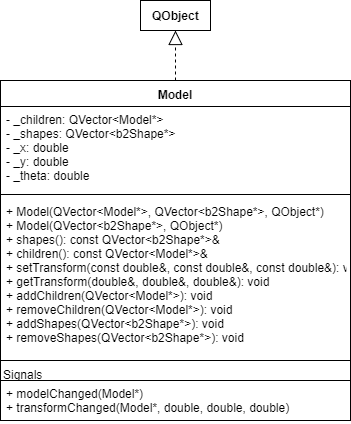
\includegraphics[scale=0.5]{./images_design/uml/Model}
 	\caption{UML of Model\label{uml:model}}
 	\end{center}
 \end{figure}  
 
 All children of a Model should exist on the heap. Upon its deletion, the Model will delete all of its children. The shapes of a Model may exist anywhere in memory, as the Model will NOT delete its shapes at any time. 
 
After construction, shapes and children models can be added and removed with the four functions
 \begin{itemize}
 	\item addChildren()
 	\item removeChildren()
 	\item addShapes()
 	\item removeShapes()
 \end{itemize} 
 
 Calling any of these functions will result in the modelChanged() signal being emitted. This design allows the UI to do the minimum amount of re-rendering necessary when part of a model updates. If the renderer needs to know when to update based on children of the model, it should use the children() method to get the list of children and listen for the modelChanged() signal from each of them.
 
 The transform of the model can be accessed through getTransform() and setTransform(). Setting the transform will result in the transformChanged() signal being emitted.
 
 Figure \ref{uml:dataflow_model} depicts the series of notifications which result from moving or modifying a Model and its child Models.
 \begin{figure}[h]
 	\begin{center}
 	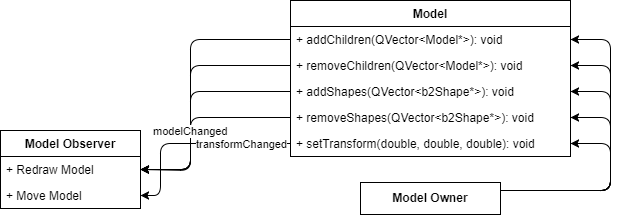
\includegraphics[width=0.75\textwidth]{./images_design/uml/DataFlow_Model}
 	\caption{Flow of data using Models. When the Model owner updates a model, any observers are notified. \label{uml:dataflow_model}}
 	\end{center}
 \end{figure}   
 
 \subsubsection*{Property}
 	Properties are variables within an object that may be modified by external sources. They are accessed through PropertyView objects, which enforce read/write rules so that internal state that should not be changed is not changed by accident. The UML Diagrams for Properties, PropertyViews, and all associated types are found in Figure \ref{uml:property}
 	
 \begin{figure}[h!]
 	\begin{center}
 	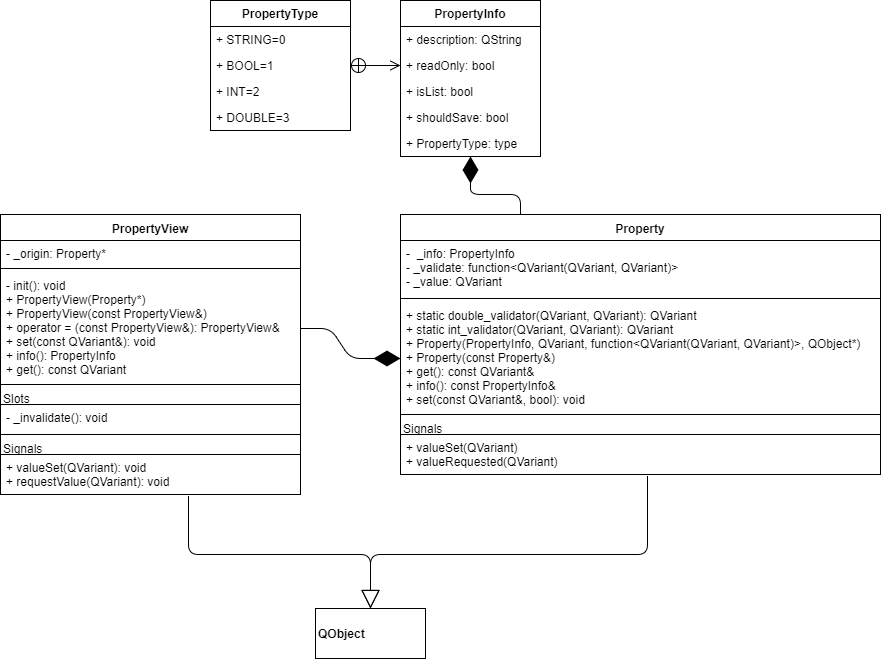
\includegraphics[width=\textwidth]{./images_design/uml/Property}
 	\caption{UML of Property and associated classes\label{uml:property}}
 	\end{center}
 \end{figure} 
 
 	A Property has three main parts
 	\begin{itemize}
 		\item Its PropertyInfo
 		\item A validation function
 		\item Its value
 	\end{itemize}
 	
 	The PropertyInfo is a container for any meta information about the Property. This contains data such as the type of the data, whether or not it's read-only, whether or not it's a list, whether or not it's required to rebuild the component, and a description of what the Property is used for. This is intended to be used to aid a UI which displays Properties to the user. It is assigned to a Property once, at construction, and can be accessed through the info() method.
 	
 	The validation function follows the prototype \lstinline|function<QVariant(QVariant, QVariant)>| and is used to make sure that the data assigned to the Property is valid. The first parameter represents the previous value, and the second parameter is a potential new value. The function should return the new value if it is acceptable and the old value if the new one is not acceptable (Optionally, the function may change the new value to make it valid and then return it). The default validation function accepts all values. A number of basic validation functions exist as static methods of the Property class for convenience. Some of them are
 	\begin{itemize}
 		\item double\_validator()
 		\item int\_validator()
 	\end{itemize}
 	
 	The value of a property is accessed and mutated though the methods set() and get(). get() returns the current value. set() validates a new value using the validation function and stores whatever value is returned. Whenever the set() function is called, the valueSet() signal is emitted with the value that was set. This happens even if the stored value does not change. The valueRequested() signal is emitted under similar conditions, but only when the value changed because of a request from a PropertyView. This can be used by the owner to only react to external changes, allowing internal changes to not trigger any slots listening for the value change.
 	
 	The PropertyView object contains all of the same public functions as a Property; however it is constructed with only a Property, which it observes. When the set() function is called on a PropertyView, the requestValue() signal is emitted, and the original Property handles that signal and validates the new value. The valueSet() signal in a PropertyView is tied to the same signal in its observed property so that any owner of a PropertyView will know when the value changes.
 	
 	The internal slot \_invalidate() is called when the observed Property is destroyed to prevent a null reference. If any accessors are called after this happens, they will return default-constructed values. It is intended that the owner of a PropertyView will receive some indication that the PropertyView should no longer be tracked from another source.
 	
 	Figure \ref{uml:dataflow_property} shows the flow of data between properties, property owners, property views, and property observers.
 	
 \begin{figure}[h]
 	\begin{center}
 	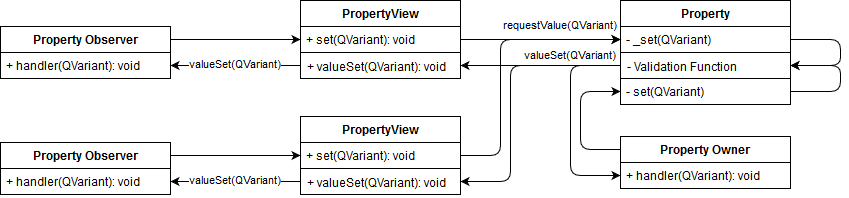
\includegraphics[scale=0.5]{./images_design/uml/DataFlow_Property}
 	\caption{Data flow of Properties, their owners, and their observers. Note that any time a value is set (Either through a PropertyView or directly) the data is validated before the new value is sent to the owner and any observers.\label{uml:dataflow_property}}
 	\end{center}
 \end{figure} 
 	
  \subsubsection*{World Object Component\label{sec:worldobjclass}}
	The main data type in this simulation is the World Object Component. For the UML diagram of a World Object Component, see Figure \ref{uml:worldcomponent_if}.
	
 \begin{figure}[h]
 	\begin{center}
 	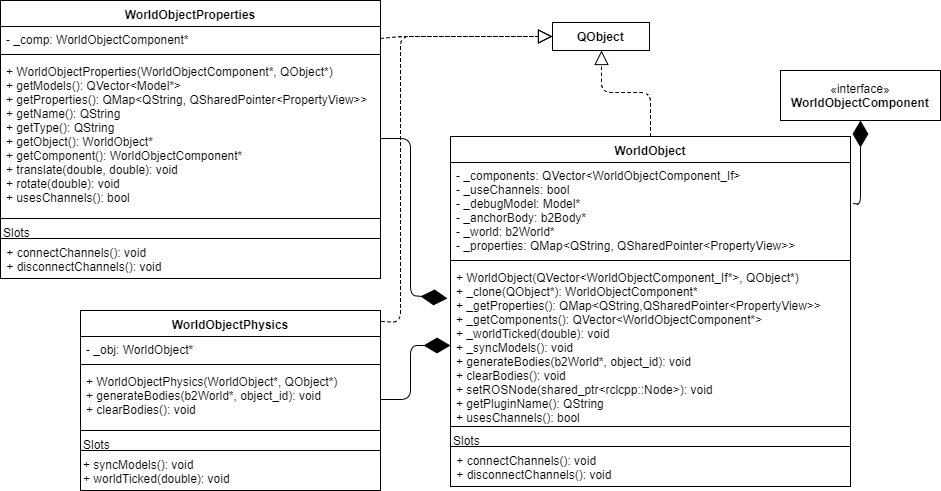
\includegraphics[scale=0.5]{./images_design/uml/WorldObj}
 	\caption{UML of World Objects, World Object Components, and associated classes\label{uml:worldobj}}
 	\end{center}
 \end{figure}
	
	It is possible that a World Object Component will use external communications, such as ROS. The usesChannels() accessor is used to determine if this is the case, and the connectChannels() and disconnectChannels() slots are used to start or stop communications.
	
	When a World Object Component is added to the physics engine, it is given access to the Box2D world. At this point, the World Object Component creates any Box2D bodies needed and set up the shapes, masses, and joints required to simulate the component. During the simulation, components can apply forces to their bodies to create movement in the world. When the World Object Component is removed from the physics engine it should destroy any joints and bodies that it has created in the current box2d world.

	The World Object Component type contains a number of methods to help integrate with the rest of the application. The main concerns are keeping track of the Models and Bodies associated with the Component and moving them around as a group when the Component is translated
	or rotated. To aid this, the methods \lstinline|registerBody()|, \lstinline|unregisterBody()|, \lstinline|registerModel()|, and \lstinline|unregisterModel()| exist as part of World Object Component. Any subclass can call these methods to add or remove handling for bodies and models. Registering either a Model or Box2D Body will move them into global space. The current transform of the Model or Body at the time of registration is assumed to be the location of that Model or Body relative to the Component (or their location in local space); upon registration, the Model or Body is moved to global space. When Bodies are registered, they can be tied to any number of Models; tying a Body to a Model means that the Model's global transform will be updated each step to match that of the Body. Bodies can also be set as the main body for the component, which means that it's location will be the location reported for the Component. If no main body is set, the Component will behave no differently, except that its location will not change due to the simulation.

	When registering and unregistering Models and Bodies, there are a couple of things to keep in mind:
	\begin{itemize}
		\item All Models should be registered during the constructor; the set of registered models should not change except during destruction
		\item Models tied to bodies are not required to be registered, and vice-versa; however, Models not tied to bodies will not move automatically, it will be up to the Component to move them during \lstinline|_syncModels()|
		\item Models and Bodies should not be destroyed until they are unregistered
		\item Models should not be destroyed while they are tied to a body
	\end{itemize}

	World Object Components also have a couple of default Properties: Name, Local X, Y, Theta, and Global X, Y, Theta. Local position is relative to any parent components; if no parent exists, then the Local position will be 0, 0, 0 at all times.

	Finally, World Object Components have a type which is assigned during construction and accessed through \lstinline|getType()|. This value is used to sort components into groups of like components.
  
	\begin{figure}
		\begin{center}
		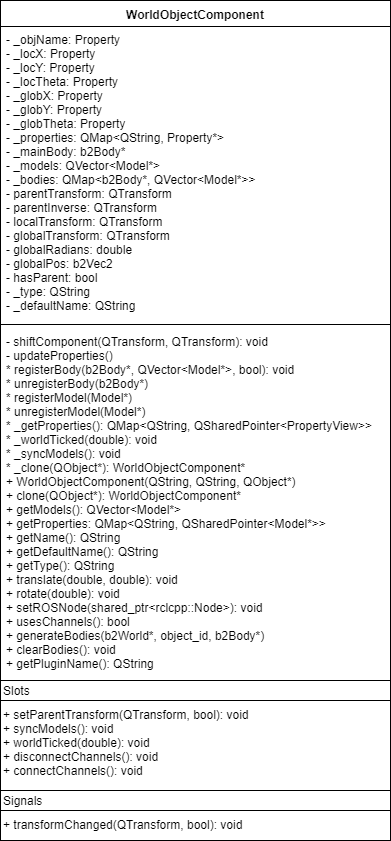
\includegraphics[scale=0.5]{./images_design/uml/WorldComponent_If}
		\caption{UML of World Component class interface\label{uml:worldcomponent_if}}
		\end{center}
	\end{figure} 

\subsubsection*{World Object}
	World Objects are a special kind of World Object Component. They are container types which hold any number of other components as children. These consolidations are the data type which is added to and removed from the simulation.

	World Objects, upon construction, consolidate all of the models and properties of their components. When getModels() or getProperties() is used to access the World Object, these consolidated lists are returned.

	Only the Simulator Core holds the reference to a World Object in the simulation. As can be seen in the UML diagram, a number of wrapper objects exist to provide specific interfaces. The WorldObjectProperties class provides an interface to a World Object which is used by the User Interface, and the WorldObjectPhysics provides the interface used by the Physics Engine. These interfaces are children (in the Qt sense) of the original World Object, so no owner of an interface needs to delete their interface when the WorldObject is removed from the simulation.
  
  \subsection{Interfaces}
  \subsubsection*{Physics Engine Interface}
  The SimulationPhysics\_If interface (UML Figure \ref{uml:phys_if}) provides the interface any Physics Engine used in this simulation must follow. It is expected that any Physics Engine will be built on Box2D.
  
 \begin{figure}[h]
 	\begin{center}
 	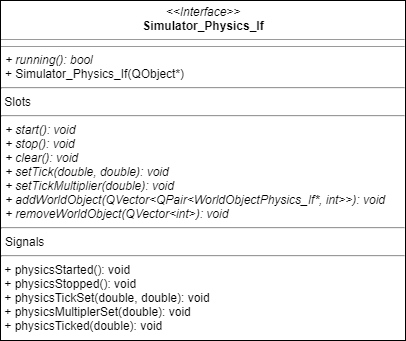
\includegraphics[scale=0.5]{./images_design/uml/Physics_Engine_If}
 	\caption{UML of Physics Engine class interface\label{uml:phys_if}}
 	\end{center}
 \end{figure}  
  
  There are four main methods for modifying the flow of the simulation and two main methods for influencing what is actually simulated.
  
  The methods for changing simulation flow are
  \begin{itemize}
  	\item start()
  	\item stop()
  	\item clear()
	\item setTick()
	\item setTickMultiplier()
  \end{itemize}
  
  The methods for adding and removing simulated objects are
  \begin{itemize}
  	\item addWorldObject()
  	\item removeWorldObject()
  \end{itemize}
  
  The Physics Engine should emit the following signals under appropriate circumstances.
  \begin{itemize}
  	\item physicsStarted()
  	\item physicsStopped()
  	\item physicsTickSet()
  \end{itemize}
  
  \subsubsection*{UI Interface}
  A UI for this simulation is expected to provide users with the following features
  \begin{itemize}
  	\item Add/Remove elements from the simulation
  	\item Start/Stop/Time Warp the simulation
  	\item Display Error messages
  \end{itemize}
  
  The UML diagram of this interface (Figure \ref{uml:ui_if}) defines the exact signals and slots that are expected for these functions.
 \begin{figure}[h]
 	\begin{center}
 	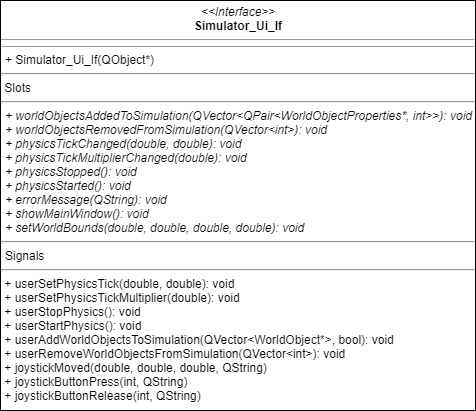
\includegraphics[scale=0.5]{./images_design/uml/Ui_If}
 	\caption{UML of UI class interface\label{uml:ui_if}}
 	\end{center}
 \end{figure}
 
 All data flow with the UI should follow a circular pattern. This means that, when the UI generates a signal, it should not update until a response has been received. This prevents the UI from getting out of sync with the rest of the application. This is the explanation for each signal having a corresponding slot. The UI should emit the signal and only update the screen when the slot is called.
 	
  \subsubsection*{View Widget Interface}
  The View Widget interface is a requirement of the specific UI written for this project. It provides a standardized way for the MainWindow UI class to update the world view widget, regardless of what drawing library that widget uses.
  
  This interface provides methods which allow
  \begin{itemize}
  	\item Setting the size of the world
  	\item Adding and removing models associated with an object
  	\item Changing how models for an object are drawn
  	\item Selecting objects and indicating selection
  \end{itemize}
  
  As with the general UI interface, the Visual Widget should not update the selected object when the user click event happens, but instead should signal that the user selected an object and wait for the objectSelected() method call.
 \begin{figure}[h]
 	\begin{center}
 	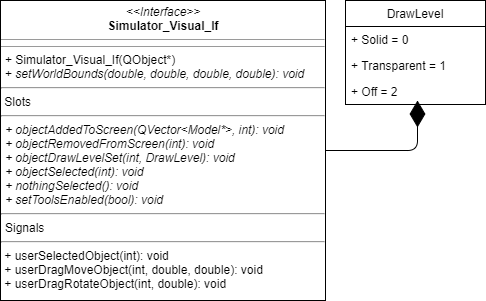
\includegraphics[scale=0.5]{./images_design/uml/Visual_If}
 	\caption{UML of Visualization widget interface\label{uml:visual_if}}
 	\end{center}
 \end{figure}
  \subsubsection*{File Handler Plugin Interface}
  File Handlers are loaded at runtime from plugin libraries following this interface. The interface should provide a set of Loaders and a set of Savers, but one or both sets can be empty. File Handler Plugins are specific to the handling of single objects or entire simulations, covered by the \lstinline|WorldObjectFileHandler_Plugin_If| and \lstinline|WorldFileHandler_Plugin_If| respectively. The loaders and savers returned by the plugin also cover the same category of files.
   \begin{figure}
 	\begin{center}
 	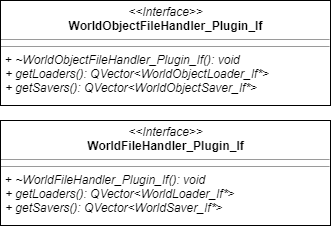
\includegraphics[scale=0.5]{./images_design/uml/FileHandler_If}
 	\caption{UML of File Handler interface\label{uml:filehandle_if}}
 	\end{center}
 \end{figure}
 File Loaders (Figure \ref{uml:fileload_if}) allow a three step process when loading files:
 \begin{enumerate}
	\item Check that a file is the proper format
	\item Prompt the user for settings
	\item Load the file, using the settings from the most recent prompt
 \end{enumerate}
 These steps are covered by the three methods of a file loader:
 \begin{enumerate}
	\item \lstinline|canLoadFile()|
	\item \lstinline|getUserOptions()|
	\item \lstinline|loadFile()|
 \end{enumerate}
 During the first step, the loader should verify that the file exists and read enough of it to determine that it is the correct format. Simply checking for the correct extension is not enough.

 If the loader needs to get information from the user to load the file, this can be done with a dialog prompt in the second step. It should not be done in the third step, because that step may not be run in the main thread.

 In the third step, the loader should open the file and load any WorldObject(s) found. The user settings chosen in the most recent prompt from \lstinline|getUserOptions()| should be used, if any are needed.

 During any of these steps, it is acceptable for the loader to throw an exception if unexpected situations are encountered.

 \begin{figure}[h]
	\begin{center}
	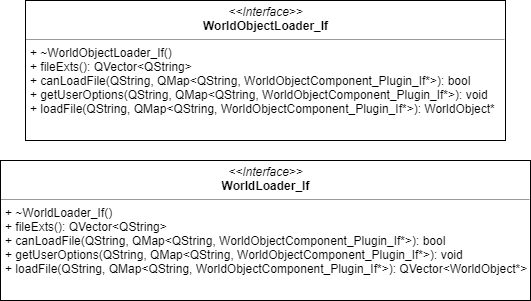
\includegraphics[scale=0.5]{./images_design/uml/Loader_If}
	\caption{UML of Plugin interface\label{uml:fileload_if}}
	\end{center}
\end{figure} 

 File Savers (Figure \ref{uml:filesave_if}) are much simpler, they have a single \lstinline|saveFile()| method which writes out the requested file.

 \begin{figure}[h]
	\begin{center}
	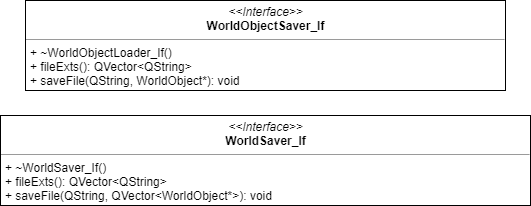
\includegraphics[scale=0.5]{./images_design/uml/Saver_If}
	\caption{UML of Plugin interface\label{uml:filesave_if}}
	\end{center}
\end{figure}

 Both File Savers and Loaders have the \lstinline|fileExts()| method which returns a vector of strings. Each of these strings should be a single group of file types that go together, following the Qt File Dialog format. For example, a file loader that can load any image file might return \lstinline|"Images (*.jpg *.png *.bmp)"|, and one that can process JSON or XML files might return \lstinline|"JSON Files (*.json)"| and \lstinline|"XML Files (*.xml)"|.

  \subsubsection*{World Object Component Plugin Interface}
  This interface defines how plugins containing World Object Components should look. Plugins are loaded using the Qt Plugin Loader; information on the plugin system can be found at \href{http://doc.qt.io/qt-5/plugins-howto.html#the-low-level-api-extending-qt-applications}{http://doc.qt.io/qt-5/plugins-howto.html}. 
  The only purpose of these plugins is to create instances of the World Object Component they contain. These instances will be cloned or added into World Objects.
 \begin{figure}[h]
 	\begin{center}
 	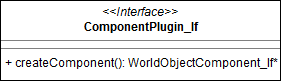
\includegraphics[scale=0.5]{./images_design/uml/ComponentPlugin}
 	\caption{UML of Plugin interface\label{uml:componentplugin}}
 	\end{center}
 \end{figure} 
 
 \subsection{Data Flow}
 All data flows between the major system components through Qt Signals and Slots. There are four main events which drive data flow
 \begin{itemize}
 	\item World Object Added
 	\item World Object Removed
 	\item Simulation Ticked
 	\item Plugin Receives External Input
 \end{itemize}
 
 \subsubsection*{World Object Added}
 	World Object additions are generally initiated by the UI. When the user wants to add an Object to the simulation, the UI signals to the core indicating what Object should be added. The core copies the World Object and stores the copy with an index. The Object and its index are sent back to the UI and Physics engine wrapped in interfaces which can be used to access methods of the new World Object.
 	
 	\begin{figure}[h]
 		\centering
 		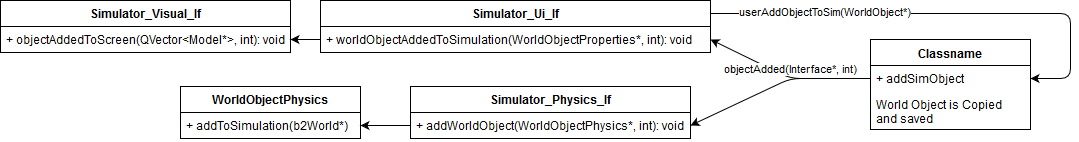
\includegraphics[width=\textwidth]{./images_design/uml/event_addObject}
 		\caption{Data flow when a new object is added to the simulation\label{uml:addevent}}
 	\end{figure}
 	
 	When the Physics engine receives a new World Object, it passes the b2World object
of the simulation to it so that the Object can add bodies and shapes to the physics engine.

	When the UI receives a new World Object, it passes the object's Model to the world view to be drawn and caches the list of object Properties. When the user selects this Object, those Properties are displayed for viewing and editing.
	
 \subsubsection*{World Object Removed}
 The process of removing a World Object is very similar to that of creating one. The UI signals to the core that the user would like to remove an Object; this Object is identified by the index that was assigned when it was added to the simulation. The core then signals back to the UI and Physics that this Object is removed and deletes the associated Object from the heap.
 
 	\begin{figure}[h]
 		\centering
 		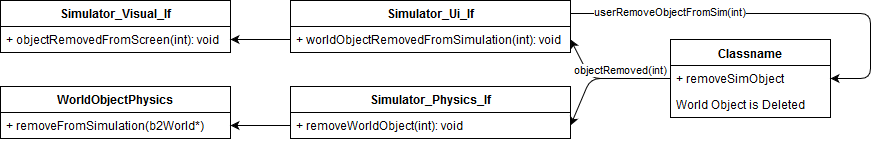
\includegraphics[width=\textwidth]{./images_design/uml/event_removeObject}
 		\caption{Data flow when an object is removed from the simulation\label{uml:removeevent}}
 	\end{figure} 
 
 When the Physics engine receives this signal, it passes the b2World to the Object again so that the Object can remove any Box2D bodies and joints that it created.
 
 When the UI receives this signal, it un-caches the Object's list of Properties and notifies the world view widget to stop drawing the Models associated with the object.
 
 \subsubsection*{World Ticked}
 World ticks are generated by the physics engine on a timer. The default tick rate is 30 per second, and each tick moves the simulation forward $\frac{1}{30}$ of a second.
 
 When a Component of an Object receives this signal, it may update its own Model, which would redraw the screen with the change. Additionally, Components can take this moment to modify the simulation by applying forces on their Box2D bodies or send messages to external applications through ROS.
 
  	\begin{figure}[h]
 		\centering
 		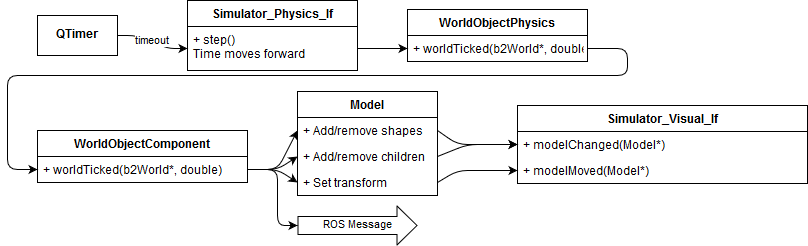
\includegraphics[width=\textwidth]{./images_design/uml/event_tick}
 		\caption{Data flow of a simulation tick\label{uml:tickevent}}
 	\end{figure}
 
 \subsubsection*{External Communication}
 The most common example of external communication is robot control code signaling that wheel velocities should change. When World Object Components receive an external communication of this nature, they can apply forces on their associated Box2D body to affect the simulation and update their models. This change will be applied on the next tick to happen after the force is applied.
 
  	\begin{figure}[h]
 		\centering
 		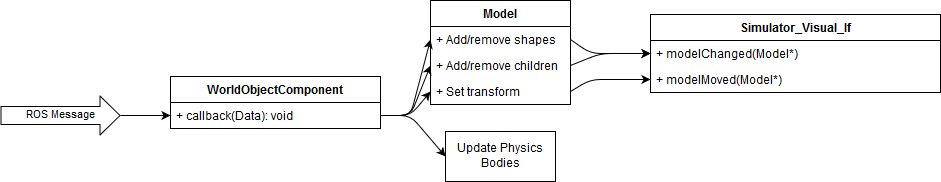
\includegraphics[width=\textwidth]{./images_design/uml/event_data}
 		\caption{Data flow of a ROS message being received\label{uml:dataevent}}
 	\end{figure}
 
\subsection{Simulator Core}

\subsubsection*{Technologies Used}
\begin{itemize}
	\item Qt
\end{itemize}

\subsubsection*{Overview}
The simulator core is, as the name suggests, the main piece of the simulation. It organizes the other parts of the system and ensures that data flows in the correct paths. The main purpose of the simulator core is to connect the UI to the Physics engine and keep them synchronized so that what's shown on screen reflects what's simulated in the physics engine. See UML Figure \ref{uml:simcore} for a list of data members and functions in the simulator core. The specific data connections set up by the core are shown in Figure \ref{uml:dataflow_simcore}.

The simulator core is also responsible for publishing timestamp messages and joystick messages. The timestamp message is, by default, published on the channel \lstinline|"roboScience/simulator/timestamp"|. It consists of a \lstinline|Float64MultiArray| with 2 values in it; the first is the total amount of time simulated since the start of the application, and the second is the amount of time simulated during the most recent tick. This message is published each time the simulation ticks. The joystick messages are the standard \lstinline|sensor_msgs/msg/joy| message provided in ROS. The channels that these messages are published on are assigned by the user
or the UI as part of the virtual joystick tool.
 
 \begin{figure}[h]
 	\begin{center}
 	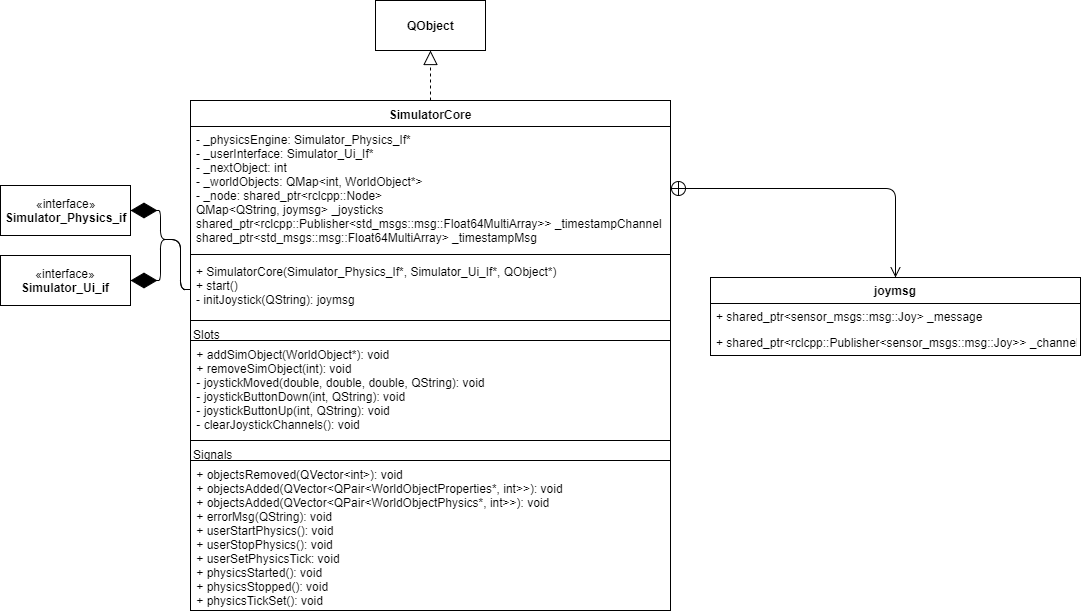
\includegraphics[width=\textwidth]{./images_design/uml/SimCore}
 	\caption{UML of Simulator Core\label{uml:simcore}}
 	\end{center}
 \end{figure}

 \begin{figure}[h]
 	\begin{center}
 	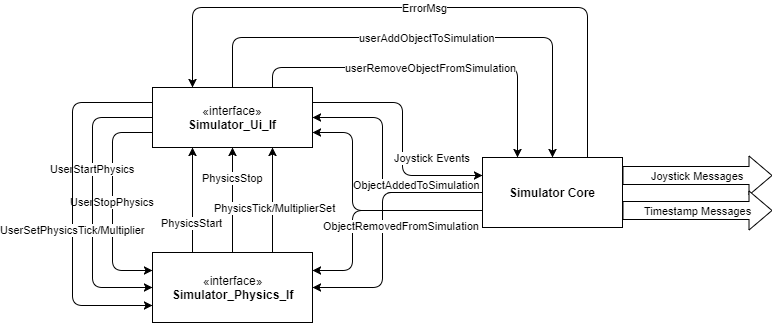
\includegraphics[scale=0.5]{./images_design/uml/DataFlow_simcore}
 	\caption{Data connections created by the Simulator Core\label{uml:dataflow_simcore}}
 	\end{center}
 \end{figure} 

\subsubsection*{Design Details}
\begin{itemize}
	\item World Objects are assigned an unsigned index when they are added. These indexes count up from 1. 0 can safely be used elsewhere as a placeholder for None.
	\item Added World Objects can be either cloned or taken by the Simulator Core. Which happens is a function of the second parameter to the \lstinline|addWorldObject()| call.
	\item The Simulator\_Ui\_If* and Simulator\_Physics\_If* that are used to construct the core will be deleted by the core's destructor.
	\item During runtime, if a new channel is requested, it will be created. The existing cache of joystick channels will be cleared when the simulation is stopped to prevent the cache from
	taking too much memory.
	\item The Simulator Core will delete the Physics and UI interfaces upon destruction, along with all existing World Objects.
\end{itemize}

\subsection{Physics Engine}

\subsubsection*{Technologies  Used}
\begin{itemize}
	\item Qt
	\item Box2D
\end{itemize}

\subsubsection*{Component  Overview}
The physics engine is responsible for updating the world state at regular intervals. When objects are first added to the world, they should be initialized in the physics engine, and until they are removed from the world they should be simulated along with the rest of the objects. The physics engine should be capable of starting, stopping, changing rate, and adding or removing an object while in any state. The current physics engine is the 'BasicPhysics' object found in UML Figure \ref{uml:physics}. The interface that it follows is found in UML Figure \ref{uml:phys_if}

 \begin{figure}[h]
 	\begin{center}
 	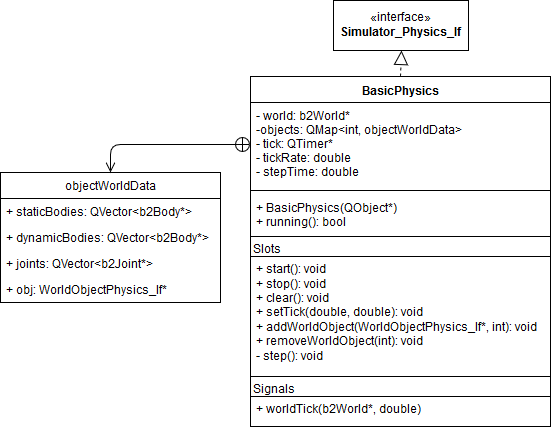
\includegraphics[scale=0.5]{./images_design/uml/BasicPhysics}
 	\caption{UML of Physics Engine\label{uml:physics}}
 	\end{center}
 \end{figure}

 \begin{figure}
 	\begin{center}
 	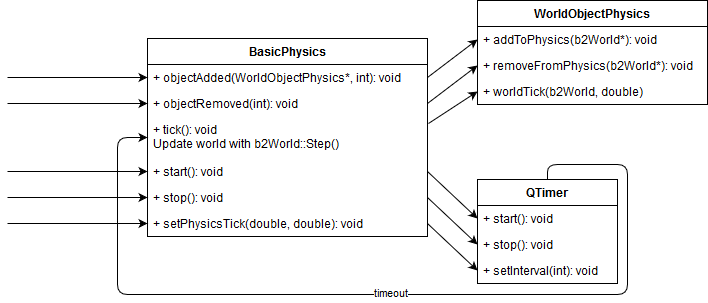
\includegraphics[scale=0.5]{./images_design/uml/DataFlow_physics}
 	\caption{Data Flow in Physics Engine\label{uml:dataflow_physics}}
 	\end{center}
 \end{figure}

\subsubsection*{Design Details}
\begin{itemize}
	\item Two things happen on every tick: The world updates (b2World::Step), then all world objects are notified of the tick. World Objects are notified twice, once through \lstinline|worldTicked()| to update internal state, and once through \lstinline|syncModels()| to update their visual representations.
	\item The QTimer is started and stopped with QTimer::start, QTimer::stop. This means that if processing a tick takes longer than the set interval, the timer events will start to stack up. It may be necessary to look at a different method of ticking to prevent this.
\end{itemize}

\subsection{User Interface}
\subsubsection*{Technologies Used}
\begin{itemize}
	\item Qt
	\item Qt Widgets
	\item Qt Custom Widgets
\end{itemize}
\subsubsection*{Overview}
The user interface implemented for this project has the following features:
\begin{itemize}
	\item Start/Stop simulation
	\item Time Warp simulation
	\item "Quick" Load/Save simulation state
	\item Load images as triangulated list of world objects
	\item Save a screenshot of the simulation
	\item Create a joystick for a robot
	\item Load/Save simulation/designer object to file
	\item New (clear) simulation/designer
	\item Designer/Simulator build widget, featuring:
	\begin{itemize}
		\item List of available world objects/components
		\item Add/Remove world object/component
		\item Export object from designer to simulation
		\item Active objects list
		\item Selected object properties
	\end{itemize}
\end{itemize}

 \begin{figure}
 	\begin{center}
 	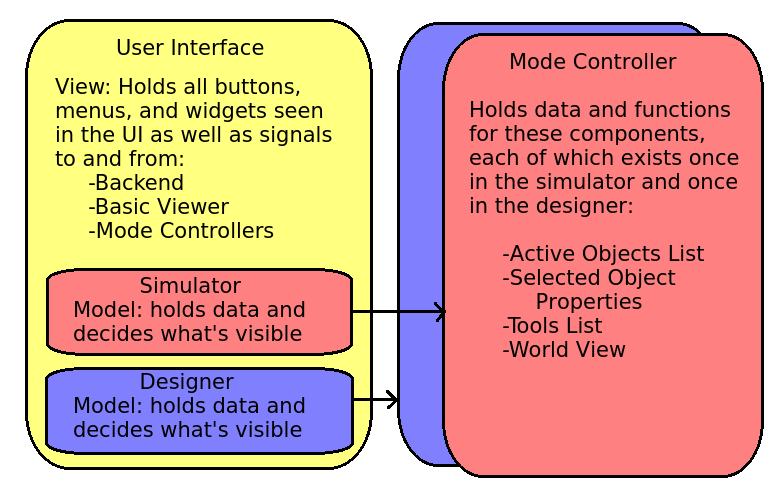
\includegraphics[width=\textwidth]{./images_design/ui_architecture.png}
 	\caption{MVC Design for the UI.\label{uml:dataflow_ui}}
 	\end{center}
 \end{figure} 
 
 \begin{figure}
 	\begin{center}
 	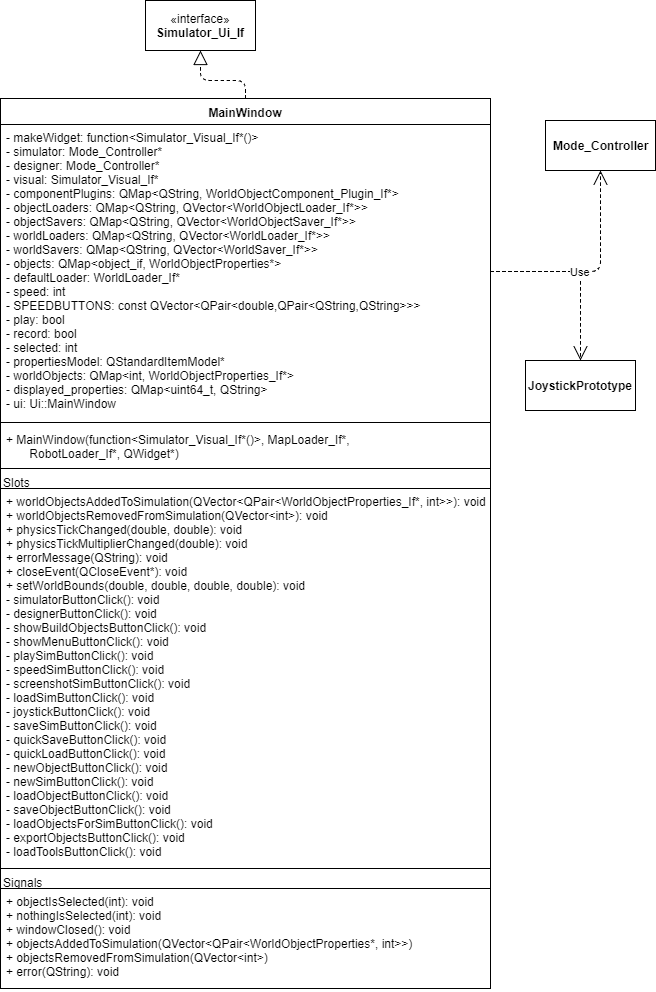
\includegraphics[scale=0.5]{./images_design/uml/MainWindow}
 	\caption{UML of User Interface\label{uml:mainwin}}
 	\end{center}
 \end{figure}

 \begin{figure}
 	\begin{center}
 	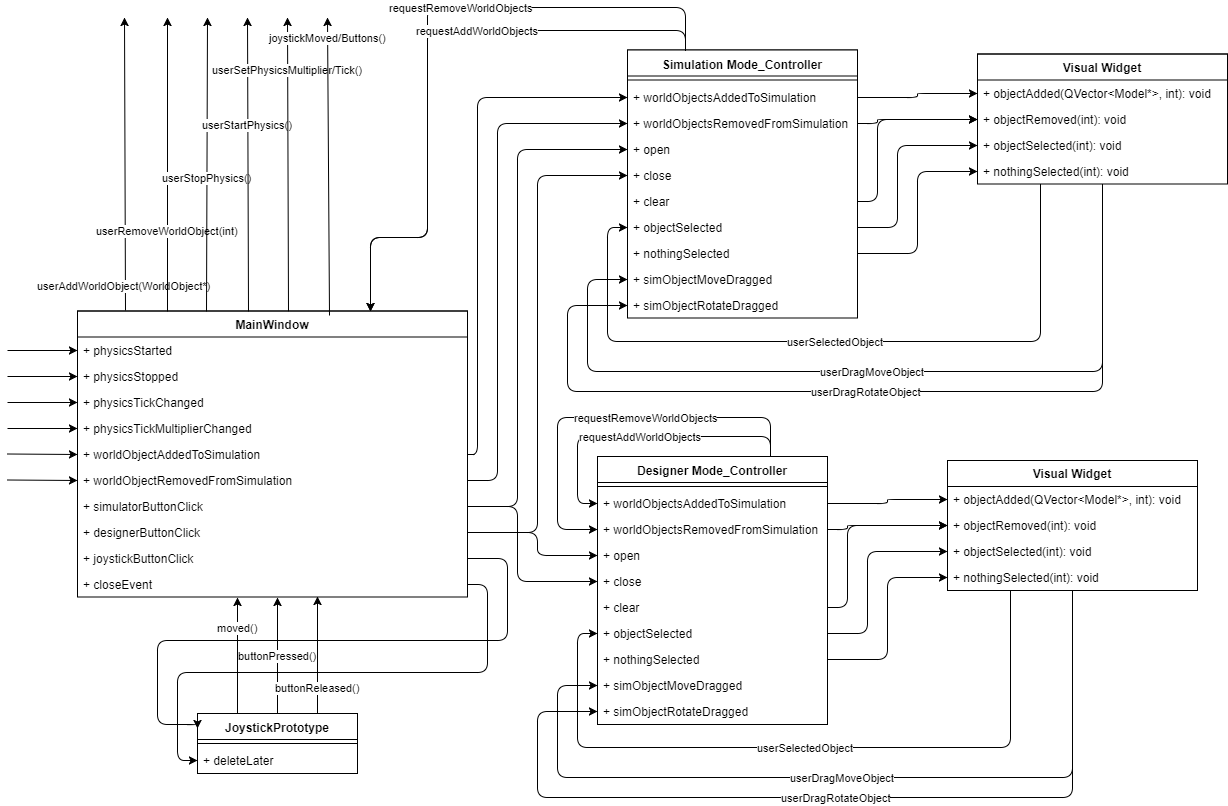
\includegraphics[width=\textwidth]{./images_design/uml/DataFlow_UI}
 	\caption{Data flow of User Interface\label{uml:dataflow_ui}}
 	\end{center}
 \end{figure} 
 
 \subsubsection*{Layout}
  \begin{figure}[h!]
 	\begin{center}
 	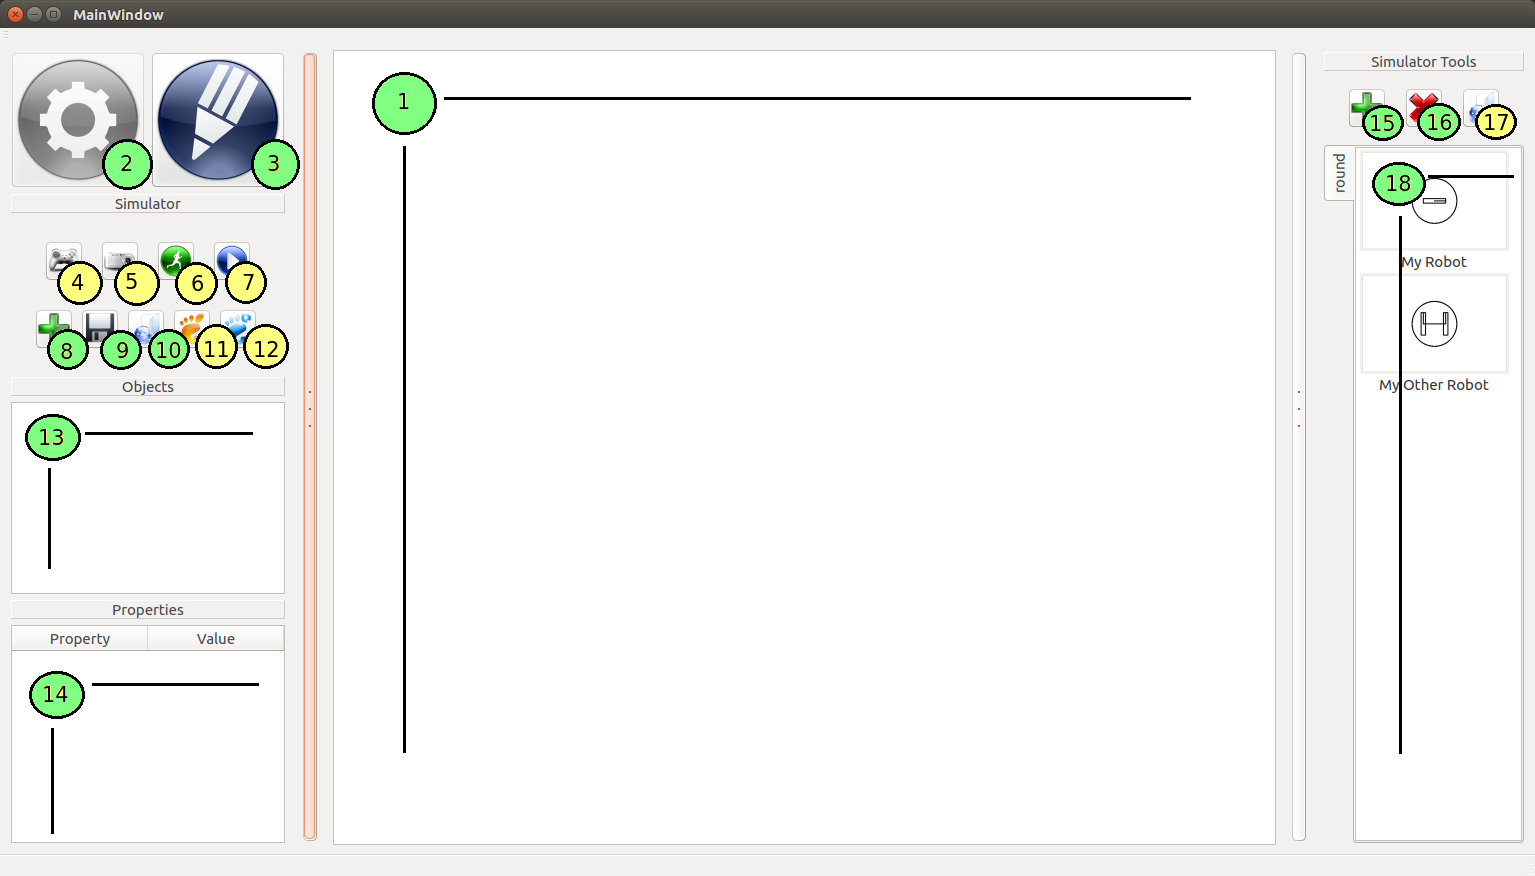
\includegraphics[width=\textwidth]{./images_design/simulator_with_my_robots_nums.png}
 	\caption{Layout of the User Interface in Simulation Mode\label{fig:sim_overview}}
 	\end{center}
 \end{figure}
 
  \begin{figure}[h!]
 	\begin{center}
 	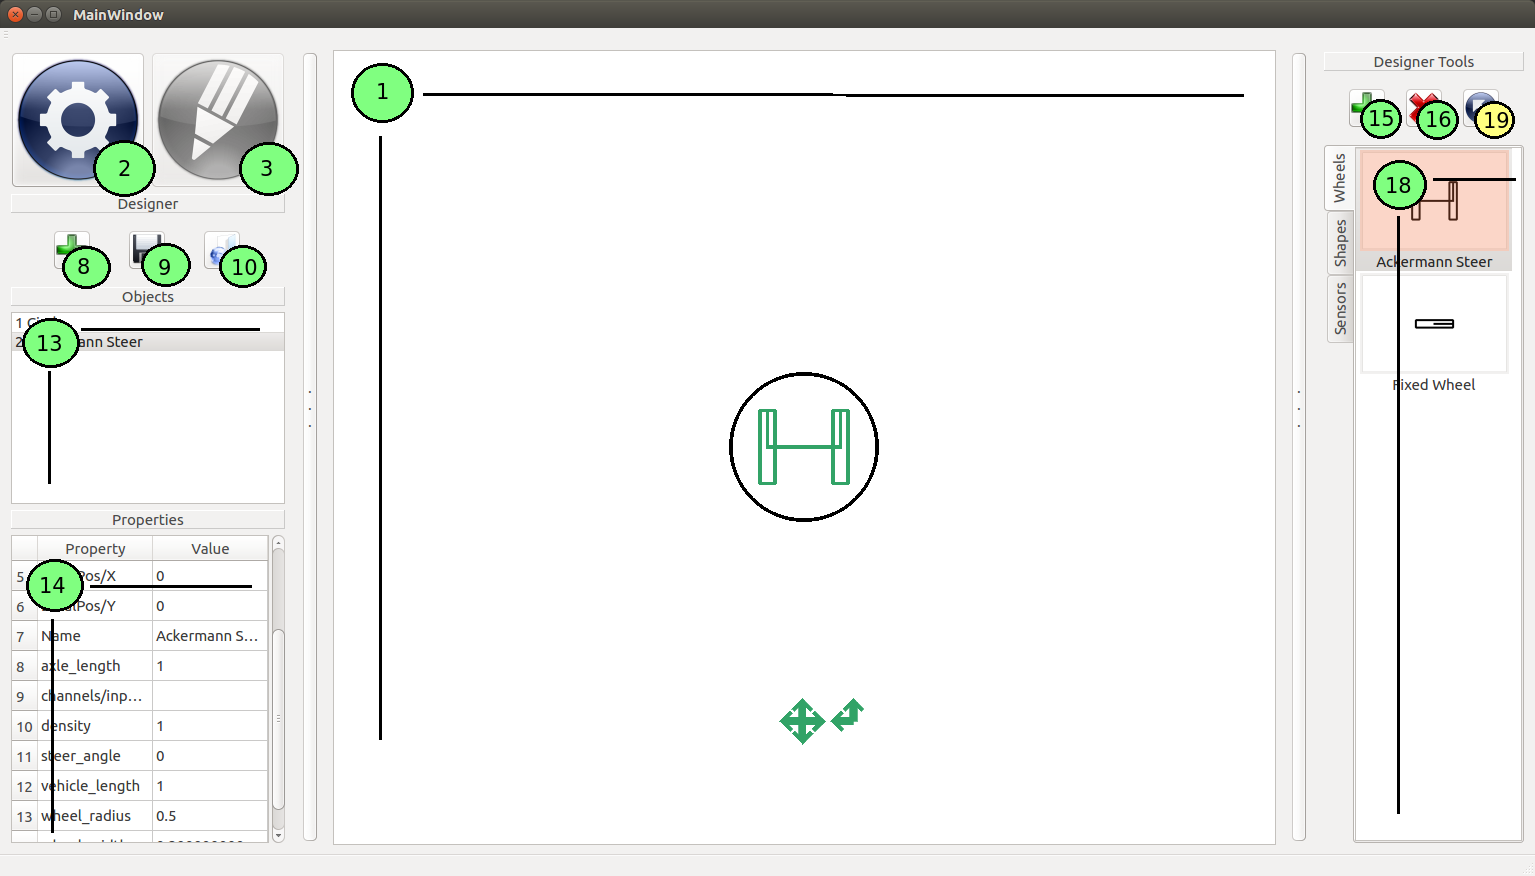
\includegraphics[width=\textwidth]{./images_design/designer_robot_creation_nums.png}
 	\caption{Layout of the User Interface in Designer Mode\label{fig:des_overview}}
 	\end{center}
 \end{figure}
 
Brief descriptions of the widgets in the UI. The UI is broken into two mode controller objects, the designer and the simulator. Both are pictured here. Widgets labelled in green appear on both the designer and the simulator, whereas those labelled in yellow are specific to only one. These descriptions are in reference to figures \ref{fig:sim_overview} and \ref{fig:des_overview}.
 \begin{enumerate}
 	\item World View Widget\\
 	Simulator: Shows what's currently happening in the simulation, any robots or world objects that have been added.\\
 	Designer: Shows the world object that's currently being designed. Pictured here, the user is designing a circular robot with Ackermann steering.\\
 	\item Simulator Mode Button\\
 	Sets the visible menus and widgets to those hosted by the simulator mode controller object. Technically only clickable when in designer mode.\\
 	\item Designer Mode Button\\
 	Sets the visible menus and widgets to those hosted by the designer mode controller object. Technically only clickable when in simulator mode.\\
 	\item Joystick Button\\
 	Opens a joystick window, where a user can select a channel to listen to and drive a robot.\\
 	\item Screenshot Button\\
 	Takes a screenshot of only the world view with no border, size dependent on the size of the world view at current time. The image will be taken without any flash or noise and automatically given a name based on systime.\\
 	\item Time Warp Button\\
 	Changes the time warping of the simulation. Current speed settings are x1, x2, x3, and x1/2.\\
 	\item Play/Pause Button\\
 	Plays or pauses the simulation. This feature combines with the Quick save/load such that a user can "restart" a simulation from any state during the course of the simulation.\\
 	\item New Button\\
 	Simulator: Clears all robots and world objects from the view and active objects list. A new simulation has no selected object.\\
 	Designer: Clears all components from the view and active objects list. A new designer object has no selected object.\\
 	\item Save Button\\
 	Simulator: Saves the simulation setup.\\
 	Designer: Saves the designer object. This does not make the designer object available for the simulation to use, that can only be done with the Export World Object Button.\\
 	\item Load Button\\
 	Simulator: Loads a simulation setup.\\
 	Designer: Loads a designer object. This does not make the designer object available for the simulation to use, that can only be done with the Export World Object Button.\\
 	\item Quick Save Button\\
 	Saves the state of the simulation when paused.\\
 	\item Quick Load Button\\
 	Loads the saved state of the simulation.\\
 	\item Active Objects List\\
 	Simulator: Shows the active objects in the simulation. These can be robots, loaded map objects, or other world objects.\\
 	Designer: Shows the components in the designer.\\
 	\item Selected Object Priorities List\\
 	Simulator: Shows the properties of the selected object. This can be a robot, a loaded map object, or another world object.\\
 	Designer: Shows the properties of the selected component.\\
 	\item Add Object/Component Button\\
 	Simulator: Makes a copy of the selected world object (item) from the tools list and adds it to the simulation.\\
 	Designer: Makes a copy of the selected component from the tools list and adds it to the designer.\\
 	\item Delete Object/Component Button\\
 	Simulator: Deletes the selected world object from the simulator view and active objects list, as well as its backend models.\\
 	Designer: Deletes the selected component from the designer view and active objects list.\\
 	\item Load World Object Button\\
 	Opens a file select to choose world object files to add to the tools list.\\
 	\item Tools List\\
 	Simulator: Shows all world objects that have been added with either the Export World Object Button in the designer or the Load World Object Button in the simulator.\\
 	Designer: Shows all components available to this user. Components are loaded at runtime and to add more, the user must download the plugin and restart the RoboScience Simulator.\\
 	\item Export World Object Button\\
 	Compiles the active components in the designer as a single world object, which becomes available to use in the simulator. The user will be prompted to give their creation a name and type.\\ 	
 \end{enumerate}
 
 \subsubsection*{Design Details}
 \begin{itemize}
 	\item All events that affect the simulation backend (the physics or core) follow a circular data path. The UI generates an event and emits it $\rightarrow$ The affected object receives the event, acts on it, and sends a response $\rightarrow$ The UI receives that response and updates so the user knows what happened.
 	\item Object properties are shown through a Model-View controller. When an object is selected, its properties are loaded into the model and connected to the dataChanged signals it emits. When the user changes the data in the model, the property views read the new data and attempt to set it on the original Property object if the property is read-only.
 	\item The UI is constructed with a factory function for making the world view widget. This can be done because the widget follows a specific interface and allows for rewriting the world view without changing any of the rest of the application.
	\item BUG: Currently, the user can change a read-only property on screen (this does not change the original property value, but the screen shows incorrect data); if they try to change a property name, the application terminates unexpectedly
	\item Since much of the functionality between the Designer and Simulator modes is shared, a common \\ \lstinline|Mode_Controller| type exists to handle properties lists, objects groups, and toolboxes.
 \end{itemize}
\subsection{World View}
\subsubsection*{Technologies Used}
\begin{itemize}
	\item Qt
	\item Qt Widgets
	\item Qt Graphics Framework
	\item Box2D
\end{itemize}
\subsubsection*{Overview}
The world viewer widget implemented in this project is called 'BasicViewer'. It uses the Qt Graphics Framework to create a 2D drawing canvas. The UML diagram for this class can be seen in Figure \ref{uml:viewwidget}.

The UI can draw things on the widget by passing it a set of Models along with an integer reference. This reference could be the identifier of a World Object which the models represent, or it could be assigned by the UI. When the UI wants to change how this set of models is drawn, or remove them from the screen, this identifying value is used.
The options for how a shape is drawn include 'selected' or 'not selected', and 'solid', 'transparent', and 'not drawn'. Only one object (group of shapes with a single identifier) may be selected at a time.
 \begin{figure}
 	\begin{center}
 	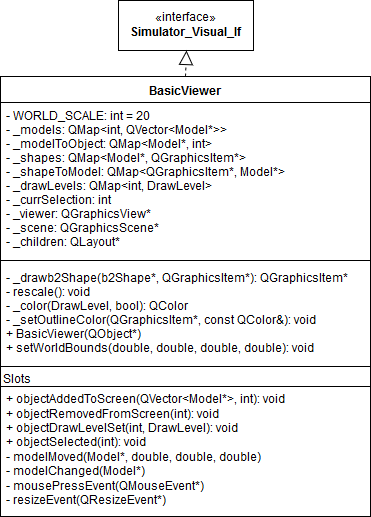
\includegraphics[scale=0.5]{./images_design/uml/BasicViewer}
 	\caption{UML of Visualization widget\label{uml:viewwidget}}
 	\end{center}
 \end{figure}
 
\subsubsection*{Design Details}
\begin{itemize}
	\item The viewer supports drawing any Box2D Shape type except for the b2ChainShape. 
	\item The widget contains both the QGraphicsScene and QGraphicsView internally. It lays out the QGraphicsView to fill itself completely on instantiation.
	\item The QGraphicsView::fitInView method appears to be broken in Qt 5.5, so the BasicView widget manually sets the viewport when it resizes.
	\item Rather than redraw an entire model when one of its children changes or moves, the widget connects to the signals of all the child models and just redraws the portions that change or move

\subsection{The main() Function}
\subsubsection*{Technologies Used}
\begin{itemize}
	\item Qt
	\item ROS
\end{itemize}

\subsubsection*{Overview}
The main() function serves a couple of important purposes.
\begin{enumerate}
	\item Create QApplication. This runs the event loop and represents the application as a whole.
	\item Start a timer to call \lstinline|rclcpp::spin_some()| at 100 hz
	\item Connect the ros spin timer to the QApplication
	\item Load all valid plugins that can be found in \lstinline|../|
	\item Instantiate a system object for each interface
	\begin{itemize}
		\item ObjectFileHandler\_If
		\item Factory function for Simulator\_Visual\_If
		\item Simulator\_Physics\_If
		\item Simulator\_Ui\_If
	\end{itemize}
	\item Instantiate and start the Simulator Core
	\item Start the Qt Event Loop
\end{enumerate}

\subsubsection*{Design Details}
\begin{itemize}
	\item Originally, the \lstinline|rclcpp::spin_some()| call was just \lstinline|rclcpp::spin()| running in a separate thread. This is the preferable setup, but ROS 2 does not handle thread-safety correctly as of the time of this project, so using a timer is a temporary solution. This results in odd behaviors when exiting the application sometimes.
	\item The directory above the executable is checked for plugins because that is, by default, where Ament places shared libraries
\end{itemize}

\section{Using the Timestamp message}
As mentioned previously, the simulator publishes a timestamp message containing both the delta time for the most recent tick and the total time passed in the simulation. This message can be used to make control code more accurate when it relies on dead reckoning. To make using this data easier, the python SimTimer class in included with the project. The SimTimer has two simple methods:
\begin{enumerate}
	\item \lstinline|double global_time()| - Returns total number of seconds
	\item \lstinline|void create_timer(delta, callback)| - Starts calling [callback] every [delta] seconds.
\end{enumerate}

Depending on its initialization parameters, the SimTimer will either listen to the simulator messages for its timestamp, in which case the global time will be the total time reported in those messages, or use a ROS node to create a repeating timer, in which case the global time will be seconds since epoch.

The SimTimer type can be included in python projects with \begin{lstlisting}
from veranda.SimTimer import SimTimer
\end{lstlisting}

SimTimer is constructed with three parameters:
\begin{itemize}
	\item useSimulatedTime: bool - Whether or not the timer should use the timestamps from the simulation. If False, the os clock will be used through a ROS node
	\item simulatedTimeChannel: string - ROS topic to listen on for timestamp messages
	\item rosNode: rclpy.Node - The ROS node to use for listening to messages and registering a normal timer
\end{itemize}

When listening to the timestamp messages, the SimTimer keeps a priority queue of all callbacks. They are ordered by their next target activation times. Each time a timestamp is recieved, it is compared to the front of the queue, and until that first item has a higher activation time than the current time, items are dequeued, called, and queued again with a higher activation time. Activation time is calculated by adding the callback delta to the time that the callback should have been called in a perfect simulation, which may differ slightly from the time that it was actually called.

\section{Plugins}
One of the main advantages to the design of this project is that it can be extended through WorldObjectComponent Plugins and FileHandler Plugins. Unfortunately, because it is a ROS package, the project (and any such plugins) must be built with Ament and CMake. A number of plugins have been included with the project to provide basic functionalities, and those plugins can be used as examples of how other plugins should be set up; however, not all plugins will follow the same patterns, so this section will describe the existing plugins as well as some of the requirements to build and use a plugin.

\subsection{Shape Plugins}
Shape plugins create a solid mass of a specific shape.

\subsubsection*{Rectangle Plugin}
The Rectangle Plugin creates a rectangular shape. The width and height
can be specified. The corresponding Properties can be found in Table \ref{tab:rectangle_props}.

\begin{table}[h!]
	\centering
	\caption{Properties exposed by the Rectangle plugin}
	\label{tab:rectangle_props}
	\begin{tabular}{c|c|c}
	Property Name & Data Type & Description\\ \hline \hline
	width & Double & Width of the rectangle (meters)\\ \hline
	Height & Double & Height of the rectangle (meters)
	\end{tabular}
\end{table}

\subsubsection*{Circle Plugin}
The Circle Plugin creates a circle shape. The radius
can be specified. The corresponding Properties can be found in Table \ref{tab:circle_props}.

\begin{table}[h!]
	\centering
	\caption{Properties exposed by the Circle plugin}
	\label{tab:circle_props}
	\begin{tabular}{c|c|c}
	Property Name & Data Type & Description\\ \hline \hline
	radius & Double & Radius of the circle (meters)
	\end{tabular}
\end{table}

\subsubsection*{Polygon Plugin\label{sec:polygon}}
The Polygon Plugin can be used to create a solid mass in any arbitrary shape, which could have holes in it. It is not intended to be added to objects manually, but should be
used by other plugins to create specifically shaped masses. In the future, it may be possible to add a polygon and modify its points, but at the time of this writing, it is not possible. Finally, the components created by this plugin are anchored and will not move in the physics engine. The properties available from a Polygon component are shown in Table \ref{tab:polygon_props}.

\paragraph{Design Details}
\begin{enumerate}
\item The Box2D polygon type does not work properly with concave polygon and has a limitation on how many points can be in a polygon. To prevent either of these limitations from being a problem, the polygon is triangulated and all of the triangles are loaded as separate shapes. The triangulation algorithm is provided by the OpenGL GLU Tesselator.
\item Polygons are simplified according to the straightness property setting. The simplification algorithm can be found in Algorithm \ref{algo:straighten}; this algorithm is called with the straightness value as its cross product threshold.
\item Triangulation is performed each time the straightness property or one of the scaling properties changes.
\end{enumerate}

\begin{table}[h!]
	\centering
	\caption{Properties exposed by the Polygon plugin}
	\label{tab:polygon_props}
	\begin{tabular}{c|c|c}
	Property Name & Data Type & Description\\ \hline \hline
	polygon\_count & Integer & Read Only: The number of triangles produced in triangulation\\ \hline
	outer\_shape & List of Points & The points that make up the outer loop of the shape.\\ \hline
	inner\_shape & List of Lists of Points & The loops of points making up the holes in the outer shape.\\ \hline
	straightness & Integer $ > 0 $ & Threshold for cross product in the simplification algorithm\\ \hline
	scale/horiz & Double & Horizontal scaling factor\\ \hline
	scale/vert & Double & Vertical scaling factor  
	\end{tabular}
\end{table}

\begin{algorithm}
\begin{algorithmic}
	\STATE{Given loop of points p and double threshold}
	\IF{Points in p <= 3} \STATE{Return p} \ENDIF
	\STATE{Let out be the output polygon}
	\STATE{Let indexA be 0}
	\COMMENT{Indices for the edges being considered}
	\STATE{Let indexB be 1}
	\STATE{Let indexC be 2}
	\STATE{Let lastCorner be false}
	\COMMENT{Set some flags and create sentinel}
	\STATE{Let firstPoint be true}
	\STATE{Let firstIndex be 0}
	\WHILE{true}
		\STATE{Let cProd be the cross product between the edges with points in p at indexA, indexB and indexA, indexC}
		\IF{cProd greather than threshold}
			\STATE{Let indexA be indexB}
			\IF{indexA is not the firstIndex}
				\STATE{Add the point in p at indexA to out}
			\ENDIF
			\IF{lastCorner is true} \STATE{break} \ENDIF
			\IF{firstPoint is true}
				\STATE{Let firstPoint be false}
				\STATE{Let firstIndex be indexA}
				\COMMENT{Set sentinel to the first point used in the output}
			\ENDIF
		\ENDIF
		\STATE{Increment indexB and mod size of p}
		\STATE{Increment indexC and mod size of p}
		\IF{indexB equals firstPoint} \STATE{Let lastCorner be true} \COMMENT{Set flag to end if we get back to the first point that was used in the output}\ENDIF
		\IF{indexC equals indexA} \STATE{Return p} 		\COMMENT{If indexC reaches indexA, the polygon is some degenerate case that this will not simplify (such as a line)}
		\ENDIF
	\ENDWHILE
	\STATE{Return out}
\end{algorithmic}
\caption{Algorithm for simplification of line loops}
\label{algo:straighten}
\end{algorithm}

\subsection{Driving Plugins}
Driving plugins produce force to propel a world object. Perhaps they would be better named 'propulsion plugins', but they usually emulate wheel-like hardware, so we're calling them driving plugins. Box2D does not actually simulate rolling of wheels in a top-down environment, so it is all done virtually. Given the size of a wheel and its angular velocity, we can calculate its linear velocity, and apply that velocity. Similarly, given its linear velocity, we can calculate the portions of that velocity in invalid directions and negate it (for example, to prevent a wheel from slipping or sliding).

It's important to note that, at least in the built-in plugins, the forces produced are proportional to the mass of the wheels. This means that if the body of a vehicle-like object is much more massive than the wheels, the wheels will have little effect on the object. This can be compensated
for by allowing the user to tune the density of wheels so that their mass
can be tweaked and made closer to the mass of what they are moving.

\subsubsection*{Fixed Wheel Plugin}
The fixed wheel plugin emulates a single wheel which cannot rotate to face a different direction. The wheel may be driven, which means its target angular velocity can be set and it will produce force in an attempt to travel the correct linear velocity. The wheel will always produce forces to negate any movement parallel to its axle (or where the axle would be if one existed). A list of the properties exposed by the plugin can be see in in Table \ref{tab:fixedwheel_props} and the input channel specification can be found in Table \ref{tab:fixedwheel_msgs}.
\paragraph{Design Details}
\begin{itemize}
\item The code for generating the wheel shape and calculating forces that the wheel should generate is shared by the Ackermann steering plugin.
\item The width of the wheel is not used in the force calculations other than to determine the mass of the wheel. It is also used for collisions.
\end{itemize}

\begin{table}[h!]
	\centering
	\caption{Properties exposed by the Fixed Wheel plugin}
	\label{tab:fixedwheel_props}
	\begin{tabular}{c|c|c}
	Property Name & Data Type & Description\\ \hline \hline
	channels/input\_speed & String & The ROS topic to listen on for target angular velocity \\ \hline
	wheel\_radius & Double & Radius of the wheel in meters\\ \hline
	wheel\_width & Double & Width of the wheel in meters\\ \hline
	is\_driven & Bool & \makecell{Whether or not the wheel should\\ produce driving force based on the input speed}\\ \hline
	density & Double & \makecell{Density of the wheel. This can be tuned to give the\\ wheel more or less mass so it affects the object\\ it is attached to better.}
	\end{tabular}
\end{table}

\begin{table}[h!]
	\centering
	\caption{ROS Messages used by the Fixed Wheel Plugin}
	\label{tab:fixedwheel_msgs}
	\begin{tabular}{c|c|c|c}
	ROS Topic & Message Type & In/Out & Description\\ \hline \hline
	channels/[input\_channel] & std\_msgs::msg::Float32 & In & \makecell{Target angular velocity (rad/s) to simulate.\\ This information is ignored if [is\_driven] is false.}
	\end{tabular}
\end{table}

\subsubsection*{Ackermann Steering Plugin}
The Ackermann steering plugin produces two linked wheels which can be steered together and will follow the Ackermann constraint. The wheels cannot be driven, they only produce forces to negate horizontal sliding, which can be used to steer a vehicle-like object. The Properties exposed and ROS channels used can be seen in Tables \ref{tab:ackermann_props} and \ref{tab:ackermann_msgs}.

\begin{table}[h!]
	\centering
	\caption{Properties exposed by the Ackermann Steering plugin}
	\label{tab:ackermann_props}
	\begin{tabular}{c|c|c}
	Property Name & Data Type & Description\\ \hline \hline
	channels/input\_angle & String & The ROS topic to listen on for target steering angle\\ \hline
	wheel\_radius & Double & Radius of the wheels in meters\\ \hline
	wheel\_width & Double & Width of the wheels in meters\\ \hline
	axle\_length & Double & \makecell{Distance between the two wheels (meters)}\\ \hline
	vehicle\_length & Double & \makecell{Distance from the 'front axle'\\ of the object to the 'back axle'\\ to be used in the Ackermann constraint (meters)}\\ \hline
	density & Double & \makecell{Density of the wheels. This can be tuned to give the\\ wheel more or less mass so it affects the object\\ it is attached to better.}\\ \hline
	steer\_angle & Bool & \makecell{Read only property: The\\ current angle being steered to}
	\end{tabular}
\end{table}

\begin{table}[h!]
	\centering
	\caption{ROS Messages used by the Ackermann Steering Plugin}
	\label{tab:ackermann_msgs}
	\begin{tabular}{c|c|c|c}
	ROS Topic & Message Type & In/Out & Description\\ \hline \hline
	channels/input\_angle & std\_msgs::msg::Float32 & In & \makecell{Angle to steer towards, radians.\\ Will be clamped to the range [$-\frac{\pi}{2},\frac{\pi}{2}$]}
	\end{tabular}
\end{table}

\subsection{Sensor Plugins}
Sensors travel with a world object and collect information about the environment. This information is usually published to the control code through ROS messages so that the control code can react to what is happening. Sensors plugins should produce the same messages as their hardware counterparts so that any control code listening to the messages does not behave differently when the messages are produced by hardware.

\subsubsection*{GPS Sensor}
The GPS Sensor is used to return the current position of an object in the world. It publishes a ROS Pose2d message, which contains
X, Y, and Theta values. The sensor can be tuned to simulate a broken GPS which drops values, has noise, or drifts over time. The noise and drift values follow normal distributions, and the chance to drop values is uniform. When a value is dropped, NaN is published instead of the current coordinate or angle. Theta is published in radians. The properties exposed to set these 
distributions as well as specify the ROS topic can be found in table \ref{tab:gps_props}.
	
\begin{table}[h!]
	\centering
	\caption{Properties exposed by the GPS Sensor plugin}
	\label{tab:gps_props}
	\begin{tabular}{c|c|c}
	Property Name & Data Type & Description\\ \hline \hline
	channels/output\_pose & String & Topic to publish Pose2D messages on\\ \hline
	publish\_rate & double & Rate of publishing (hz)\\ \hline
	probabilities/x & double & Probability of publishing x coordinate [0.0, 1.0]\\ \hline
	probabilities/y & double & Probability of publishing y coordinate [0.0, 1.0]\\ \hline
	probabilities/theta & double & Probability of publishing theta [0.0, 1.0]\\ \hline
	drift/x/sigma & double & Variance of drift in x direction per second\\ \hline
	drift/x/mu & double & Mean of drift in x direction per second\\ \hline
	drift/y/sigma & double & Variance of drift in y direction per second\\ \hline
	drift/y/mu & double & Mean of drift in y direction per second\\ \hline
	drift/theta/sigma & double & Variance of drift in theta direction per second\\ \hline
	drift/theta/mu & double & Mean of drift in theta direction per second\\ \hline
	noise/x/sigma & double & Variance of noise in x direction\\ \hline
	noise/x/mu & double & Mean of noise in x direction\\ \hline
	noise/y/sigma & double & Variance of noise in y direction\\ \hline
	noise/y/mu & double & Mean of noise in y direction\\ \hline
	noise/theta/sigma & double & Variance of noise in theta\\ \hline
	noise/theta/mu & double & Mean of noise in theta
	\end{tabular}
\end{table}
\begin{table}[h!]
	\centering
	\caption{ROS Messages used by the GPS Plugin}
	\label{tab:gps_msgs}
	\begin{tabular}{c|c|c|c}
	ROS Topic & Message Type & In/Out & Description\\ \hline \hline
	channels/output\_channel & geometry\_msgs::msg::Pose2D & Out & \makecell{The 2D Pose message containing x, y, and theta}
	\end{tabular}
\end{table}
\paragraph{Design Details}
\begin{itemize}
	\item Drift accumulates over time even on ticks when the value is not published
	\item NaN is produced using \lstinline|std::numeric_limits<double>::quiet_NaN()|
\end{itemize}

\subsubsection*{Touch Sensor Ring}
The touch sensor ring plugin mimics a ring of touch sensors with a specific radius. It is intended to be used on circular robots, so that its radius can be set to the same as the robot. 
	The sensor ring can be set to sense a specific section of the circle, and the number of sensors used can be specified. Whenever the state of one of the buttons changes, a ROS message is published. Extra circles are drawn on the world visualization to show which touch sensors are triggered. An example of this can be seen in Figure \ref{fig:touchsensorexample}. Details of the properties exposed by the plugin and the ROS messages it utilizes can be found in tables \ref{tab:touch_ring_props} and \ref{tab:touch_ring_msgs}
	
	\begin{figure}[h]
		\centering
		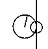
\includegraphics{./images_design/touch_sensor}
		\caption{Example of the touch sensor ring sensing something. The large circle is a robot, the small circle is the touched sensor point.}
		\label{fig:touchsensorexample}
	\end{figure}
\begin{table}[h!]
	\centering
	\caption{Properties exposed by the Touch Sensor Ring plugin}
	\label{tab:touch_ring_props}
	\begin{tabular}{c|c|c}
	Property Name & Data Type & Description\\ \hline \hline
	channels/output\_channel & String & The ROS topic to output sensor messages to\\ \hline
	angle\_start & Double (0-360) & Angle that the sensed section starts at\\ \hline
	angle\_end & Double (0-360) & Angle that the sensed section ends at\\ \hline
	ring\_radius & Double & Radius of the touch sensor ring\\ \hline
	sensor\_count & Integer & \makecell{Number of sensors spaced evenly in the slice\\ of the circle defined by angle\_start and angle\_end}
	\end{tabular}
\end{table}
\begin{table}[h!]
	\centering
	\caption{ROS Messages used by the Touch Sensor Ring Plugin}
	\label{tab:touch_ring_msgs}
	\begin{tabular}{c|c|c|c}
	ROS Topic & Message Type & In/Out & Description\\ \hline \hline
	channels/output\_channel & std\_msgs::msg::ByteMultiArray & Out & \makecell{1-Dimensional vector with one\\ element for each touch sensor on\\ the ring. Untriggered buttons\\ are set to 0, triggered\\ ones are non-0.}
	\end{tabular}
\end{table}
\paragraph{Design Details}
\begin{itemize}
	\item All the required circle shapes for the touch sensors are generated at the start. They are added to and removed from the model when they become active or inactive.
	\item The touch sensor circle is a solid physics shape which can collide. This generates collision points from Box2D that can be used to know what is sensed.
	\item The body with the sensor ring fixture is held in place relative to the robot by a Box2D Weld Joint. The ring has a very low density (so as not to affect how the robot drives) so, due to the implementation of Weld Joints,  it is possible for the ring to behave in strange ways if it is larger than the robot it surrounds. Specifically, if there is a collsion and the robot continues to drive, the robot can be seen moving around within the touch sensor ring; it does not stay anchored in the center as one might expect.
\end{itemize}
\subsubsection*{Lidar Sensor}
The lidar sensor behaves as a regular hardware lidar would. It scans an area in front of (or around) itself at a high rate and reports the distances to the objects scanned. The lidar provided by this plugin can be customized to scan any size range from 0 to 360 degrees, with the center of the range directly in front of the lidar. The number of scan rays and the radius (maximum range) can also be specified, along with the rate of scanning. Each time a scan is performed, the image representing the lidar and its scan will be updated, and a ROS message will be published. A list of An example of the lidar can be seen in Figure \ref{fig:lidarsensorexample} and the properties exposed by the sensor and its ROS messages can be found in Tables \ref{tab:lidar_props} and \ref{tab:lidar_msgs} respectively.

\begin{figure}[h]
	\centering
	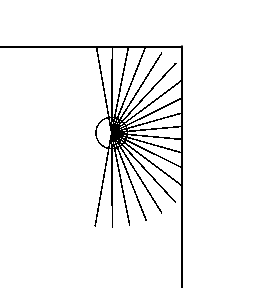
\includegraphics[scale=0.5]{./images_design/lidar_sensor}
	\caption{Example of the ldar sensor sensing something. The lidar has 20 rays in a range of 200 degrees; the rays are shortened on the sensor's left and front sides because it is in a corner.}
	\label{fig:lidarsensorexample}
\end{figure}

\paragraph{Design Details}
\begin{itemize}
\item The Box2D shapes used to represent the lidar beams are created any time a Property changes which affects them. During runtime, their lengths are modified to represent what is seen.
\item Given a range of $x$ degrees, the lidar will report beams from the angle of $-\frac{x}{2}$ to $\frac{x}{2}$, relative to the lidar body.
\item Any beams which do not detect an obstacle will report a distance of $\infty$, as defined by the implementation of \lstinline|std::numeric_limits<float32>::infinity()|.
\end{itemize}

\begin{table}[h!]
	\centering
	\caption{Properties exposed by the Lidar Sensor plugin}
	\label{tab:lidar_props}
	\begin{tabular}{c|c|c}
	Property Name & Data Type & Description\\ \hline \hline
	channels/output\_channel & String & The ROS topic to output sensor messages to\\ \hline
	scan\_range & Double (0-360) & Total angle range to sense, in Degrees\\ \hline
	scan\_radius & Double & Max distance away from the sensor to detect\\ \hline
	scan\_points & Integer $\geq$ 2 & \makecell{Number of beams spaced evenly in the range,\\ including the first and last beam.}\\ \hline
	scan\_rate & Double & Rate (hz) of scans and messages.
	\end{tabular}
\end{table}
\begin{table}[h!]
	\centering
	\caption{ROS Messages used by the Lidar Sensor Plugin}
	\label{tab:lidar_msgs}
	\begin{tabular}{c|c|c|c}
	ROS Topic & Message Type & In/Out & Description\\ \hline \hline
	channels/output\_channel & sensor\_msgs::msg::LaserScan & Out & \makecell{The standard ROS LaserScan message \\with parameters filled according to the \\property settings of the sensor.}
	\end{tabular}
\end{table}

\subsection{Image Loading Plugin}
One of the functions of the original STDR was that it could load an image, and then the dark pixels of the image would be treated as obstacles. This was simple for the STDR to do because of the way it did collision detection - on a per-pixel basis. Collisions in this project are done in the Box2D engine, so in order to provide a similar functionality, a plugin is included which converts an image to a set of obstacles which can be loaded into the physics engine. The algorithm for converting an image to polygons consists of a couple of steps, and can be found in Algorithms \ref{algo:findshapes}, \ref{algo:blackwhite}, \ref{algo:findpoints}, and \ref{algo:followbound}. The plugin can handle the common image formats .png, .jpg, and .bmp. All images are converted to black and white before processing. A threshold is chosen by the user, and all pixels with an intensity above that are changed to 255 and all pixels with intensity at or below it are set to 0. The polygons are constructed using the polygon component defined in Section \ref{sec:polygon}. When a file is loaded, the user is presented with a prompt in which they can specify the following:
\begin{enumerate}
	\item Width and height of the image (meters)
	\item Pixels per meter in both the horizontal and vertical directions
	\item Straightness value for the shapes read
	\item Greyscale threshold
\end{enumerate}

\paragraph{Design Details}
\begin{enumerate}
\item The triangulation and simplification necessary to load polygons into the physics engine is not done in the plugin, but in the polygon component type. Similarly, scaling is also done in the polygon component type.
\end{enumerate}

\begin{algorithm}
	\caption{Convert a black and white image to a set of polygons and holes}
	\label{algo:findshapes}
	\begin{algorithmic}
		\STATE{Given 2D rgb pixel array and intensity threshold}
		\STATE{Let blackAndWhite be the output from Algorithm \ref{algo:blackwhite}}
		\STATE{Let shapes be a vector of pairs of outer loops and inner loops}
		\FORALL{Values v in blackAndWhite}
			\IF{v is false (black)}
				\STATE{Perform BFS starting at v to find region of connected black pixels}
				\STATE{Create new 2D boolean array of true (white) large enough to hold the region + 1 on each side}
				\STATE{Copy region into new array}
				\STATE{Let shift be the x, y offset in img of the upper-left corner of the bounding box of the region}
				\STATE{Set all pixels in the region to be true (white) in the original image}
				\STATE{Let outer, inner be the result of running Algorithm \ref{algo:findpoints} on the copy of the region}
				\STATE{Add shift to every point in the outer loop and every point of every one of the inner loops}
				\STATE{Store outer, inner as an output shape in shapes}
			\ENDIF
		\ENDFOR
		\STATE{Return shapes}
	\end{algorithmic}
\end{algorithm}

\begin{algorithm}
	\caption{Convert an image to black and white}
	\label{algo:blackwhite}
	\begin{algorithmic}
		\STATE{Given 2D rgb pixels array img and intensity threshold}
		\STATE{Let out be a 2D boolean array with same dimensions as img}
		\FORALL{Pixels p in img}
			\IF{intensity(p) > threshold} \STATE{Let corresponding location in out be true}
			\ELSE \STATE{Let corresponding location in out be false}
			\ENDIF
		\ENDFOR
		\STATE{Return out}
	\end{algorithmic}
\end{algorithm}

\begin{algorithm}
	\caption{Convert a black and white image of a single shape to an outer loop and inner hole loops}
	\label{algo:findpoints}
	\begin{algorithmic}
		\STATE{Given 2D boolean array img}
		\STATE{Let firstEdge be false}
		\COMMENT{Used to determine if we want to move clockwise or counterclockwise when following boundaries}
		\STATE{Let out be a pair containing an empty outer loop and an empty set of inner loops}
		\FORALL{Pixels p in img}
			\IF{p is True and at least one of the four adjacent pixels to p is False}
				\STATE{Let bound be the pixels found by Algorithm \ref{algo:followbound} starting at p}
				\IF{firstEdge is true}
					\STATE{Let the outer loop of out be bound}
				\ELSE
					\STATE{Add the bound to the inner loops of out}
				\ENDIF
				\STATE{Let firstEdge be false}
				\STATE{Perform a BFS on true pixels starting at p}
				\STATE{Set every pixel found in the BFS to false}
			\ENDIF
		\ENDFOR
		\STATE{Return out}
	\end{algorithmic}
\end{algorithm}

\begin{algorithm}
	\caption{Follow the boundary between a black region and a white region}
	\label{algo:followbound}
	\begin{algorithmic}
		\STATE{Given 2D boolean array img, starting location x, y, and boolean flag clockwise}
		\STATE{Let searchNext be 0}
		\COMMENT{Indicates which point to start with when checking points around the current point. Index 0 is 1, -1 relative, 1 is 1, 0 relative, 2 is 1, 1 relative, and so on}
		\STATE{Let points be an empty list of output points}
		\STATE{Let currPoint be the start x, y}
		\STATE{Let lastPoint be currPoint}
		\REPEAT
			\STATE{Add currPoint to points}
			\STATE{Let good be false}
			\FOR{Each of the 8 points surrounding currPoint, starting with searchNext and continuing in the fasion described above (If clockwise is false, go the opposite direction). Let each point be called next}
				\IF{next is true}
					\FOR{Each neigbor f to next which is false}
						\STATE{Let cProd be the cross product between currPoint, next and currPoint, f}
						\IF{cProd is greater than 0}
							\STATE{Let good be true}
							\STATE{Let lastPoint be currPoint}
							\STATE{Let currPoint be next}
							\STATE{Let searchNext be searchNext + 4 mod 8
							\STATE{break}}
						\ENDIF
					\ENDFOR
				\ENDIF
			\ENDFOR
		\UNTIL{currPoint equals start}
		\STATE{Return points}
	\end{algorithmic}
\end{algorithm}

\subsection{The JSON Plugin}
One general-purpose file handler plugin is provided as part of the project. It is able format WorldObjects and WorldObjectComponents as JSON objects which can be stored in files. The JSON formatter can be used to save single World Objects and entire Simulations.

\subsection{Custom Plugins}
Custom plugins should be ROS packages in the same workspace as the simulator package. The plugin's package.xml file should specify at least the following in order to resolve build order:
\begin{lstlisting}
<depend>veranda_api</depend>
<depend>veranda_box2d</depend>
\end{lstlisting}

Once Ament is aware of package dependencies, the CMakeLists file must be set up to find the required libraries and files and build the plugin correctly.

First, there are a number of definitions and values that need to be set in order to compile and link the Qt-Specific portions of the plugin
\begin{lstlisting}
find_package(Qt5 REQUIRED COMPONENTS
  Core Gui
)

set(CMAKE_INCLUDE_CURRENT_DIR ON)
set(CMAKE_AUTOMOC ON)

add_definitions(-DQT_PLUGIN)
add_definitions(-DQT_SHARED)

include_directories( ${CMAKE_BINARY_DIR} )
\end{lstlisting}

In order to resolve dependencies for Box2D and the header files from the simulator, find\_package needs to be called for the associated packages. Then \lstinline|include_directories| needs to be called so the Qt MOC can resolve headers
\begin{lstlisting}
find_package(veranda_api REQUIRED)
find_package(veranda_box2d REQUIRED)
    
ament_export_dependencies(
    veranda
    veranda_box2d
)

include_directories(${veranda_api_INCLUDE_DIRS})
include_directories(${veranda_box2d_INCLUDE_DIRS})
\end{lstlisting}

Next, any headers in the plugin containing the \lstinline|Q_OBJECT| or other \lstinline|Q_*| macros need to be preprocessed by the MOC
\begin{lstlisting}
	set(plugin_moc_hdrs a.h b.h ... z.h)
    qt5_wrap_cpp(MOC_SRCS ${plugin_moc_hdrs})
\end{lstlisting}

Finally, the plugin needs to be built as a shared library and linked against Qt Core libraries and the Box2D library.
\begin{lstlisting}
add_compile_options(-fPIC)

add_library([plugin name] SHARED ${CPP_SRCS} ${MOC_SRCS})
qt5_use_modules([plugin name] Core Gui)

ament_target_dependencies([plugin name]
	"veranda_box2d"
	"veranda_api"
	)
\end{lstlisting}

The last detail is that the plugin must be deployed in the directory above the simulator executable. This can be achieved by installing the plugin to the \lstinline|lib| directory of the workspace install.
\begin{lstlisting}
    install(
      TARGETS [plugin name]
      DESTINATION lib
    )
\end{lstlisting}

\subsubsection*{Other Notes}
The class types which extend the plugin interfaces will need to include either \lstinline|world_object_component_plugin.h| or \lstinline|file_handler_plugin.h|. According to ROS/Ament convention, this should be done with \lstinline|#include <veranda/[type]_plugin.h>|; however, due to a bug in the Microsoft Visual Studio Compiler, this is not a cross-platform compatible solution (It is unknown if this works using Clang on OSX). In order for the MOC to properly resolve headers and search upward in the dependency tree on Windows, the inclusion must be done using the full path, either absolute or relative: \lstinline|#include "../../../install/include/veranda/[type]_plugin.h"|. While this breaks convention and is inconvenient, it should still be a fairly modular solution which just depends on your workspace directory structure up to the plugin's folder matching that of the plugin writer's. Worst case, if you import a plugin and it does not match your directory structure, it should be simple to modify the include so the paths match.

\subsubsection*{A Note About ROS Communications}
It is believed by the project team that, because the rclcpp::spin() method may be called from a thread other than the main one, all ROS message callbacks may be run from a non-main thread. (Whether this is true or not is not known for sure, but the ROS documentation seems to indicate that it is the case.) Care should be taken when defining callbacks in components to prevent race conditions which would result from this design. This issue was resolved in the included plugins with the use of a Qt Signal and Slot. When a Qt Signal triggers a Slot of an object which resides in a different thread, the slot is queued for the second thread to receive naturally during its event loop, preventing any race conditions. The various components have an internal signal and slot specifically for this purpose; the signal is emitted by the ROS callback function, and that copies the data from the callback into the main thread where it can be processed safely.

\end{itemize}